\documentclass[oneside]{book}
\usepackage[paperwidth=17cm, paperheight=22.5cm, bottom=2.5cm, right=2.5cm]{geometry}
\usepackage{amssymb,amsmath,amsthm} %paquete para símbolo matemáticos
\usepackage[spanish]{babel}
\usepackage[utf8]{inputenc} %Paquete para escribir acentos y otros símbolos directamente
\usepackage{enumerate}
\usepackage{graphicx}
\usepackage{setspace}
\usepackage{float}
\usepackage[nottoc]{tocbibind}
\setcounter{secnumdepth}{3} %para que ponga 1.1.1.1 en subsubsecciones
\setcounter{tocdepth}{3} % para que ponga subsubsecciones en el indice
\usepackage{fancyhdr}
\renewcommand{\baselinestretch}{2}
\begin{document}
%\begin{figure}[h] %	
%	
\includegraphics[width=11cm, height=11cm]{escudo} %	
%\end{figure}
\title{El Nosotros de los pueblos zapatistas y la estructura del Átomo Social de Margaret Gilbert} %Con este nombre se guardará el proyecto en writeLaTex

\author{Fís. Gustavo Magallanes Guijón}
\date{}
\thispagestyle{empty}
\maketitle
\thispagestyle{empty}
\maketitle

\thispagestyle{empty}
\setlength{\headheight}{15pt}
\frontmatter

\chapter*{}
\begin{flushright}
    
    \textit{Espero que este trabajo pueda aportar\\ un poco más al estudio de la noción de Nosotros, \\y a la reflexión y construcción\\de relaciones intersubjetivas. }
\end{flushright}
\chapter*{Agradecimientos}

\noindent{Agradezco en primer lugar a mi directora de tesis, la Dra. María de los Ángeles Eraña Lagos quien me acompañó  y me orientó sobre las lecturas que seguí a lo largo de este trabajo. Muchas gracias Ángeles.}

Agradezco a la Dra. Mayte Muñoz por las observaciones que hizo al texto y sus valiosas opiniones al respecto. También estoy muy agradecido con la Dra. Fernanda Navarro por haber discutido sobre el pensamiento del filósofo Carlos Lenkersdorf, así como con el Dr. Miguel Hernández y el Dr. Ambrosio Velasco por haber revisado con atención esta propuesta.

        Mi familia ha estado presente en la elaboración de este trabajo. Su apoyo y su aliento fueron el motor para seguir adelante.
\\
\\
\\
\\

        No puedo dejar de lado a todos y a todas mis amigos que me acompañaron en todos estos días en la construcción de este trabajo: Claudia Guerrero Robledo, Yenifef Dianaild López Jaramillo, y muchos más que han estado presentes en las discusiones en torno al concepto de Nosotros.

        A los alumnos del Seminario de Ciencia y Sociedad de la Facultad de Ciencias con quiénes discutí y enriquecí mis opiniones sobre el Nosotros. A todos los seminaristas, gracias.

        Finalmente, no quiero dejar de lado que la fuente para iniciar esta tesis fueron las palabras de los pueblos zapatistas y su recurrente apología del Nosotros. Esto me llevó a reflexionar sobre la pertiencia de este concepto no sólo en la vida social y política, sino en el ámbito de la filosofía. Espero poder contribuir con este trabajo en esa dirección. 
    
¡Muchas gracias a todos!
\pagestyle{fancy}
\fancyhf{}
\lhead[\textit{\small{\rightmark}}]{\textit{\small{\rightmark}}}
\rhead[\thepage]{\thepage}

\fancyhead[lo]{\slshape\nouppercase{\rightmark}}
\fancyhead[re]{\slshape\nouppercase{\leftmark}}

\lfoot[\tiny{\textit{Gustavo Magallanes Guijón}}]{\tiny{\textit{Gustavo Magallanes Guijón}}}
\rfoot[\tiny{\textit{El Nosotros de los pueblos zapatistas\\ y la estructura del Átomo Social de Margaret Gilbert}}]{\tiny{\textit{El Nosotros de los pueblos zapatistas\\ y la estructura del Átomo Social de Margaret Gilbert}}}
\renewcommand{\footrulewidth}{0.5pt}
\tableofcontents
\setcounter{tocdepth}{3} % para que ponga subsubsecciones en el indice
\mainmatter %empieza la numeración de las páginas

\chapter*{Introducción}
\addcontentsline{toc}{chapter}{Introducción}
\markboth{Introducción}{Introducción} % encabezado 
\noindent{En la historia de las ideas, la noción del Yo ha sido importante en la formulación de conceptos y razonamientos que han trascendido en ámbitos políticos, científicos y filosóficos. Así ocurrió por ejemplo con las reflexiones del pensador René Descartes, quien sostuvo que el principio intuitivo del pensamiento racional radicaba en el \textit{Yo}\cite{Descartes}, o como con las ideas de David Hume las cuales reducían esta noción a un haz de percepciones\cite{Hume}}.

Con el avance de la modernidad, la noción del Yo permeó la ciencia política, la psicología, la economía y demás áreas del conocimiento. Esto es notorio, por ejemplo en la psiquiatría con las teorías psicoanalíticas de Sigmund Freud\cite{Freud}, y en la filosofía política con el liberalismo inglés iniciado por John Locke\cite{Locke}. Sin lugar a dudas esta noción ha sido importante en la historia y ha dado lugar a debates y discusiones que seguramente se siguen estudiando a la fecha.\\

Desde el ámbito de la filosofía también se ha pensado, discutido y teorizado respecto a la noción de \textit{Nosotros}. Y en esta reflexión han debatido pensadores contemporáneos de relevancia como el inglés John Searle, la estadounidense Margaret Gilbert, el finlandés Raimo Tuomela, el irlandés Phillip Pettit, el filósofo y lingüista alemán Carlos Lenkersdorf, así como los filósofos mexicanos Fernanda Navarro y Luis Villoro Toranzo.

Esta discusión aún no es cabal y aún se sigue escribiendo y debatiendo al respecto. Y este trabajo intenta seguir este debate sugiriendo una noción de Nosotros soportada por el pensamiento de Carlos Lenkersdorf  y sobre todo aterrizada en las palabras de los pueblos zapatistas.

Esto será fundamental en el desarrollo de esta tesis, ya que el objetivo se centrará en trabajar una propuesta de Nosotros trazada a partir de la palabra y en señalar la potencia de la misma. 

Dicho concepto me es de interés porque frente a nuestros tiempos tanto la noción de Yo como la de Nosotros es conveniente revisarlas y analizarlas con el fin de entender nuestro presente desde el ámbito filosófico.

Pero también porque estoy convencido de que la comprensión de las entidades colectivas: sus estructuras y atributos nos puede ayudar a seguir reflexionando en términos de filosofía de la ciencia. Esto desde la epistemología colectiva, sus problemas y su relación con otras áreas del conocimiento, así como la constante revisión de conceptos tales como: intención colectiva. 

Esto sin dejar de lado que algunos otros temas de interes para la filosofía de la ciencia, y para la filosofía en esta dirección, son discusiones que van desde el organicismo o bio-organicismo hasta aquellos tópicos que versan sobre problemas filosóficos, políticos y sociales en torno a inteligencia artificial en sistemas agenciales.

En este trabajo, el estudio de las entidades colectivas lo realizo desde el análisis de la palabra de un grupo organizado, del Ejército Zapatista de Liberación Nacional, en el que sus participantes hablan lenguas distintas y pertenecen a culturas diferentes, pero comparten intereses, deseos y formas de trabajo.

De modo que la noción de Nosotros que presento se basa fundamentalmente en la palabra, en lo que se dice y aquello que se predica. Esta es la razón por la cual me di a la tarea de estudiar las entidades colectivas desde el enfoque de Margaret Gilbert y el de Carlos Lenkersdorf, pues estos dos autores examinan las palabras y oraciones sin dejar de lado su acción lingüística. 

Así, pensando en el lenguaje como hilo conductor, analizaré la noción de \textit{átomo social} de Margaret Gilbert quien discute las entidades colectivas desde su forma más simple: la relación entre dos personas para luego pensarlas en cantidades mayores. 

Este análisis me ayuda a configurar el Nosotros que propongo a partir del análisis del \textit{compromiso conjunto}, pues como expondré, su persistencia ayuda a mantener (o no) la cohesión de la entidad colectiva.

El estudio del pensamiento de Margaret Gilbert es pertinente porque la filósofa realiza la reflexión desde el examen de la acción lingüística de oraciones del orden común, lo cual me sirve para continuar la propuesta pero desde las ideas de Carlos Lenkersdorf quien señala que a través del análisis de lo que se dice día a día en los pueblos tojolabales se puede configurar un Nosotros de carácter  \textit{intersubjetivo}.

El trabajo de Carlos Lenkersdorf es de gran ayuda, en primer lugar porque fue una persona cercana a las comunidades zapatistas, entendió la cosmovisión de estos pueblos y sus relaciones sociales desde la filosofía y la lengua, por lo que me parece pertinente desarrollar mi propuesta apoyándome en sus reflexiones. 

Siguiendo con la configuración de mi propuesta, es pertinente el trabajo de Luis Villoro, pues además de que conoció de cerca los pueblos zapatistas y fue estudioso de los pueblos indios, su noción de \textit{comunitarismo} me ayuda a entender este Nosotros.


No está de más decir que mi interés personal por trabajar este concepto radica en la preocupación política y social, por lo que pretendo en un futuro trabajar esta noción más cerca de la filosofía política, así que el resultado de este trabajo lo seguiré reflexionando y analizando.

Dicho lo anterior, para el desarrollo de esta tesis, en el primer capítulo expongo la propuesta de Margaret Gilbert en torno a la naturaleza de las entidades colectivas, examino la estructura del \textit{compromiso conjunto} revisando sus características y las condiciones que lo posibilitan y su vínculo con el \textit{Sujeto plural}.

En el capítulo dos examino la noción de \textit{intersubjetividad} de Carlos Lenkersdorf y en seguida el de \textit{comunitarismo} de Luis villoro. Para después plantear la propuesta que desarrollo en esta tesis, el Nosotros de los pueblos zapatistas.

La propuesta vertida en este capítulo estará soportada en los textos públicos del EZLN, las Juntas de Buen Gobierno (JBG), los Municipios Autónomos Rebeldes Zapatistas (MAREZ). 
	
En el tercer y último capítulo, establezco un diálogo entre la estructura del átomo social de Margaret Gilbert y el \textit{Nosotros}\footnote{En adelante para referirme al Nosotros de los pueblos zapatistas lo haré como Nosotros, pues en los documentos que han divulgado los zapatistas, cuando se refieren a este concepto lo hacen de esta manera.} que aquí presento. De igual manera señalo las convergencias y puntos en común entre estas nociones, así como sus divergencias.

Concluiré este trabajo mostrando que la metodología de Margaret Gilbert apoyada de un contexto social, político, etc., ayuda efectivamente a generar y configurar un Nosotros. También subrayaré la potencia de esta noción no sólo en el ámbito filosófico sino además en el político y social. 

\chapter{La estructura del Átomo Social de Margaret Gilbert}
\noindent{Cuando hablamos de \textit{átomo}, comúnmente nos referimos a la idea de que la materia en el universo está compuesta fundamentalmente por átomos, así se estableció desde el siglo V a.C. con los pensadores presocráticos Leucipo y Demócrito; y luego en la teoría atómica física de Dalton, Lavoissier y Avogadro. Sin embargo, en el campo de la sociología o ciencia política este concepto tiene múltiples significados.}

Una destacada pensadora, y de quien expondré su trabajo en este capítulo es la filósofa estadounidense Margaret Gilbert, quien analiza la noción de \textit{átomo social} y su estructura. Para lo cual aborda nociones tales como punto de permiso (o requisito de permiso), intención colectiva, acción conjunta, disponibilidad, etc., conceptos que serán de gran ayuda para estructurar el Nosotros que expodré en el capítulo siguiente. 

Así que la comprensión de estos conceptos será importante para el desarrollo de esta tesis, pues el análisis de las entidades colectivas en su simplicidad, (como por ejemplo la relación entre dos personas), aporta información teórica para comprender entidades más numerosas. 

Si bien es cierto que llevar los conceptos de esta autora a grupos más grandes tiene sus problemas, también es cierto que desde esta óptica podemos tener una aproximación a un problema molecular.

Así, problematizando con las ideas de Gilbert para la entidad más simple, después podré pasar al estudio de entidades mayores como la molécula social o el Sujeto Plural ya que contaré con un \textit{background} de instrumentos teóricos para su examen.

En el texto \textit{The Structure of the Social Atom: Joint Commitment as the Foundation of Human Social Behavior}\cite{gilbert_1}, la filósofa nos dice que si se comprende qué es un átomo social, entonces se comprende una entidad más numerosa: el \textit{Sujeto Plural.}

Como ejemplo de partida, Gilbert elige el caso de dos personas que no se conocen y tienen un primer contacto.

El ejemplo consiste en dos personas que caminan en sentido contrario sobre una calle y cruzan miradas a lo lejos (inmediatamente uno de ellos camina un poco más rápido debido a las miradas). Y ya cerca uno de ellos se dirige al otro y lo saluda con un “¡Buen día!”, lo que es en seguida contestado por la otra persona con otro “¡Buen día!”.

Gilbert analiza esta situación destacando que se ofrece información relevante para pensar la constitución del átomo social si se examina en por lo menos dos momentos: antes y después del saludo.

Antes del saludo ocurre que uno de ellos caminó más rápido ante la mirada del otro individuo, interactuaron de alguna manera. Después del saludo podríamos preguntarnos si dicha acción es ya suficiente para asegurar que estas dos personas se unifiquen y constituyan ahora un \textit{átomo social}\footnote{Margaret Gilbert se refiere al \textit{átomo social} como la unida mínima social, la cual no tiene que ver con la postura filosófica llamada \textit{atomismo} o \textit{individualismo ontológico}, en el cual se afirma que la sociedad es la suma de individuos y la suma de sus partes. Algunos autores destacados sobre esta postura son: Paul von Lilienfeld, Albert Schaffle, y René Worms. En línea en <<http://www.enciclopediadelapolitica.org>>.}.

Así, bajo el examen de lo que sucede en una situación ordinaria, de la cotidianidad, vemos que es posible obtener información relevante que puede aportar al entendimiento de la estructura del átomo social.

Además este ejemplo es interesante porque plantea la posibilidad de generar un átomo social de manera espontánea. Sin que dos personas se conozcan o hayan tenido contacto alguno.

Esta metodología es importante para la propuesta que desarrollaré más adelante, pues a partir del análisis de una situación simple extraeré información para el análisis filosófico.

\section{El compromiso conjunto}

\noindent{Uno de los conceptos clave en la teoría de Margaret Gilbert es el de compromiso conjunto. Y es clave porque bajo éste se configura y explica la noción de átomo social y luego una entidad mayor, el Sujeto plural.}
	
El compromiso conjunto también será importante en la propuesta que presento, señalaré que gracias a que hay un compromiso conjunto, es que también hay un Nosotros. 

Y cómo es clave para lo que voy a desarrollar es importante en la exposición desglosar y explicar este concepto. En este sentido Gilbert subraya elementos teóricos que permiten examinarlo y entenderlo desde su postura filosófica.

Ella menciona que en la \textit{estructura del átomo social} están presentes la \textit{acción conjunta}, el \textit{punto de permiso} y la \textit{intención colectiva} por lo que estas nociones merecen su especial atención ya que sólo con ellos se puede comprender el compromiso conjunto. A continuación expongo tales conceptos.

\subsection{Punto de permiso}
\noindent{A diferencia del ejemplo que se expuso en el apartado anterior, Gilbert nos propone una situación en la que dos personas ahora sí se conocen y comparten el gusto por salir a caminar, llegando con esto a situaciones en las que se problematiza el punto de permiso y la acción conjunta.}
	
%Ahora bien, la diferencia sustancial entre el punto de permiso y la acción conjunta, en principio no es clara. Por lo que comenzaré a explicar el punto de permiso para en seguida hacer el la exposición de la acción conjunta. Veamos.

La autora nos propone lo siguiente:

Considérense dos personas, Bill y Jane, quienes  están caminando juntos. Ahora suponga que sin advertencia, Bill rápidamente para la caminata y dice “¡Me separo!” Él entonces deja de caminar abandonando a Jane\footnote{Gilbert, Margaret. \textit{The Structure of the Social Atom: Joint Commitment as the Foundation of Human Social Behavior} en Socilaizing Methaphysics. F. S. Schmitt ed. P. 42.}.

La acción repentina de Bill podría causar alguna reacción en Jane ya sea sorpresa, decepción, o incluso pensar que el comportamiento de Bill es incorrecto y merece ser criticado o reprochado.

Gilbert reflexiona sobre la estructura lógica de lo ocurrido. Ella nos dice que si suponemos a un grupo de personas que están involucradas en una acción, y si además suponemos que uno de los miembros no tiene el permiso de los demás para abandonar la actividad, se sigue que este participante hace algo incorrecto hacia el grupo.\footnote{\textit{Ibíd}. P.42.}

Aquí surge una primera cuestión interesante para analizar y comenzar a entender el concepto de punto de permiso: 

¿Acaso se necesita obtener permiso para abandonar la actividad conjunta? Alguien  podría decir: “Bill no necesita obtener el permiso de Jane para abandonar la caminata”.

Para Gilbert, en situaciones como la expuesta siempre está presente el punto de permiso. Y no reconocer que se requiere de la autorización de las partes involucradas para abandonar la actividad, puede deberse al rechazo a reconocer que el grupo tiene algún tipo de poder sobre la conducta y decisiones individuales. O que esto provenga de la falta de un análisis suficientemente cuidadoso de la situación. De acuerdo con ella, si hiciéramos esto último veríamos que incluso para situaciones simples se requiere el \textit{punto de permiso.}

¿Es posible que se pueda presentar una situación en el que el punto de permiso esté ausente? Para Gilbert esto no es así, sino por el contrario el punto de permiso siempre está presente y permite comprender y explicar qué es lo que ocurre cuando en ciertas situaciones se abandona la actividad conjunta. 

Así, el punto de permiso ayuda a explicar aquellas situaciones en las que una parte explícitamente otorga el permiso a la otra para salir de la acción conjunta. Estos son denominados acuerdos del tipo “ad hoc”\footnote{\textit{Ibíd}. P. 43.}.

Supóngase, por ejemplo que Jane le propone a Bill caminar juntos alrededor del barrio. Bill está de acuerdo pero le advierte que no está seguro que él quiera caminar mucho. Y abre la posibilidad de abandonar la actividad.

La situación sería así:
\begin{quote}
Mira Bill, si tú quieres parar en algún punto no hay problema, yo estaré feliz de seguir la caminata sola. 

Vamos pues. ―Le responde Bill.

Y ya andando ambos en la caminata. 

Yo creo que pararé aquí ―Le dice Bill.

Adiós, entonces.―Ella le responde. 
\end{quote}

En este contexto Jane le concede explícitamente permiso a Bill para dejar la caminata. Es un acuerdo ad hoc en el que ambas partes están en sintonía para que en algún momento se pueda abandonar la acción por alguna de las partes.

Pareciera que el \textit{punto de permiso} no es necesario en este ejemplo, sin embargo sí lo es, pues Jane antes de iniciar la actividad conjunta, aceptó la decisión de Bill de abandonar el paseo en algún punto cercano. Al aceptarla, Jane otorgó permiso a Bill para dejar de caminar con ella cuando él quisiera.

Otro ejemplo para explicar la necesidad del punto de permiso puede ser el caso de dos amigos (Emiliano y Alexis) que acordaron con antelación ir al cine, pero que finalmente uno de ellos no llega a la cita.

Podría ocurrir que en una conversación anterior, Emiliano haya comentado sobre su mala memoria y falta de concentración a Alexis, insistiéndole en que si alguna vez falla, intente comprenderle. Ante tal advertencia, Alexis pudo contestarle que no se preocupara. Digamos que se otorga el permiso para abandonar la actividad conjunta. (A este tipo de acuerdo Gilbert lo llama \textit{convención privada}).

Recurramos de nuevo al caso que propuso la autora, la caminata de Bill y Jane. Ellos se conocen muy bien y disfrutan caminar juntos. Ambos saben, sin embargo, que Bill encuentra incómodo tener que pedir permiso por algo. Pero pueden haber desarrollado un entendimiento en el que cuando están en una caminata juntos, Bill puede dejar de participar sin problema. Hay una \textit{convención privada. }

Vemos que en este contexto, sí es necesario el punto de permiso para abandonar la actividad conjunta, pues hay un antecedente que permite un acuerdo entre ambos, lo cual posibilita que Bill pueda abandonar la caminata cuando lo decida.

Finalmente, las \textit{convenciones sociales} son otro tipo de situaciones en el que se puede problematizar el punto de permiso. Pensemos que la caminata se desarrolla en una sociedad en la que el hombre puede dejar de participar en el momento que él lo decida sin la autorización o permiso de la mujer. De nuevo, el punto de permiso explica si alguien deja de participar en este tipo de acción, pues el contexto social otorga el permiso dadas las normas sociales o políticas. El caso de las sociedades patriarcales como la de los judíos jaredíes, o las matriarcales como la zapoteca en Oaxaca podrían ser un marco contextual de este tipo.

\subsection{Intencionalidad colectiva}

%\noindent{Para el análisis de este concepto, partiremos del caso más simple para luego exponer el caso colectivo.}

\noindent{Cotidianamente escuchamos oraciones que refieren a intenciones colectivas, como la de “tenemos la intención de trabajar en el proyecto” o la de “intentaremos ganar el partido”. Y para el caso de una persona escuchamos frases como “estoy estudiando para sacar buenas notas” u “hoy me esforzaré por llegar más temprano, ya voy en camino”, oraciones en las que la intención de esa persona se expresa cuando ésta intenta hacer algo y, siendo guiada por la intención, se comporta de modo que pueda satisfacerla\footnote{\textit{Íbid.} P. 46.}.}

Ya sea en lo individual o en lo colectivo la intención va acompañada con una acción de por medio que podría realizarse. De modo que un planteamiento formal de la intención tiene que estar acompañada por la actividad que se pretende hacer. En este sentido, la autora nos plantea formular dicha intencionalidad sin perder de vista que lo que está directamente involucrado es una actividad a realizar. Para esto, nos propone re-elaborar el ejemplo de la caminata la siguiente manera:

\begin{quote}
Las personas A y B están caminando juntas si y sólo si intentan colectivamente caminar juntas; y si cada una de ellas actúa a la luz de esta intención colectiva, de modo que ésta esté en el proceso de ser satisfecha. Más precisamente, cada persona actúa a la luz del compromiso conjunto intentando como un cuerpo caminar juntos.\footnote{\textit{Ibíd}. P. 46.} 
\end{quote}

Lo cual se puede reformular de la siguiente manera:

\begin{quote}
Las personas A y B intentan colectivamente hacer X, si y sólo si A y B están conjuntamente comprometidos a intentar como un cuerpo hacer X\footnote{\textit{Ibíd}. P. 46.}.
\end{quote}

Considerando la expresión “intentar como un cuerpo” como a una agrupación o unión de personas que intentan colectivamente realizar un propósito.

Esto con un ejemplo quedará más claro.

Pensemos en dos personajes, Alexis y Emiliano quienes intentan realizar una tarea en colectivo. Esto significa también que Alexis y Emiliano están conjuntamente comprometidos a intentar realizar su tarea de modo que estén acorpados a modo de agrupación.

O también se puede ver de esta otra manera: Si Emiliano y Alexis están conjuntamente comprometidos en intentar como si fueran una sola entidad, ya sea colectivo o grupo realizar cierta tarea. Se cumple que ellos intentan hacer su tarea en colectivo.
\\

Vemos pues que en las intenciones colectivas hay un compromiso consigo mismo para lograrlo. Y podemos decir que cuando ellos intentan lograr propósitos u objetivos colectivos también lo hacen basándose en una intención. 

%Vemos pues que definir la intencionalidad colectiva conlleva a explorar y estudiar otros conceptos. Se abren más preguntas al respecto. Y una de ellas es el significado más de cerca del compromiso conjunto en torno al significado: “las personas están conjuntamente comprometidas”.

%Y pareciera que es algo obvio lo que se dice en dicha sentencia, pero precisamente con el análisis y el examen cuidadoso vemos que no es así, y que su definición relaciona otros conceptos que nos ayudan a seguir encontrando otros conceptos y sus vínculos.

Además queda de manifiesto que la intención colectiva y el compromiso conjunto son conceptos estrechamente ligados, por lo que también el análisis del compromiso conjunto ayudará a comprender la intencionalidad colectiva.

%Margaret Gilbert señala que la \textit{acción colectiva} se puede explicar en términos de \textit{intenciones colectivas}  

\subsection{Acción conjunta}

\noindent{Ya tenemos las piezas clave para abordar la acción conjunta: El punto de permiso, y la intencionalidad colectiva. Y lo son ya que la acción conjunta está fuertemente entrelazada con estos conceptos. Veamos.}

%Desde la noción de punto de permiso ya vimos que su propuesta no se puede entender, o estructurar la \textit{acción conjunta} sin tener en cuenta el \textit{punto de permiso.}

Se entrelaza con el punto de permiso pues como ya vimos, éste es requisito para la acción conjunta, y además este concepto ayuda a explicar algunas de las convenciones para llevar a cabo la acción conjunta como la convención \textit{ah doc} o  la \textit{privada.} 

Este entrelazamiento puede ser tan fuerte que incluso se puede perder la distinción entre un concepto y otro, o diluir las fronteras dadas las circunstancias por las que podría pasar el grupo o colectivo. De modo que tanto el punto de permiso como la acción conjunta son conceptos que pueden confundirse por lo que conviene diferenciarlos para tenerlos más claros.
\\

La distición la podemos observar de la siguiente manera: 

\textbf{La acción conjunta} puede parecer natural, como un ‘hecho bruto’ relativamente primitivo; mientras que para el caso del \textbf{requerimiento de permiso} no es así, pues este parece artificial, relativamente sofisticado, a modo de normas y valores.

Sin embargo no hay que perder de vista que ambos conceptos están entrelazados y que el uno y el otro están presentes. 

Finalmente, como se expuso en el aprtado anterior, la intencionalidad colectiva se entrelaza con la acción conjunta en el sentido de que la noción de intención colectiva se plantea como un componente necesario para la comprensión de la acción conjunta.

Tomando en cuenta estos aspectos, la definición de acción conjunta está formulada de la siguiente manera:
\begin{quote}
La acción conjunta es ``gente haciendo algo juntos, lo cual implica que tienen la intención colectiva de hacer eso juntos''.\footnote{Gilbert, Margaret. (2006). \textit{Rationality in collective action. Philosophy of the social sciences}. P. 36.}
\end{quote}

% Sacado de: Huichuan Xia, Yun Huang, Jennifer Stromer-Galley (2016):
%A Collective Action Inspired Motivation Framework for Crowdsourcing.
%In Karin Hansson, Tanja Aitamurto, Thomas Ludwig, Michael Muller (Eds.),
%International Reports on Socio-Informatics (IRSI),
%Proceedings of the CSCW 2016 – Workshop: Toward a Typology of Participation in Crowdwork
%(Vol. 13, Iss. 1, pp. 41-48)
%Margaret Gilbert. (2006): Rationality in collective action. Philosophy of the social sciences 36, 1, 2006, 3–17.

\begin{figure}[h]
	\centering
	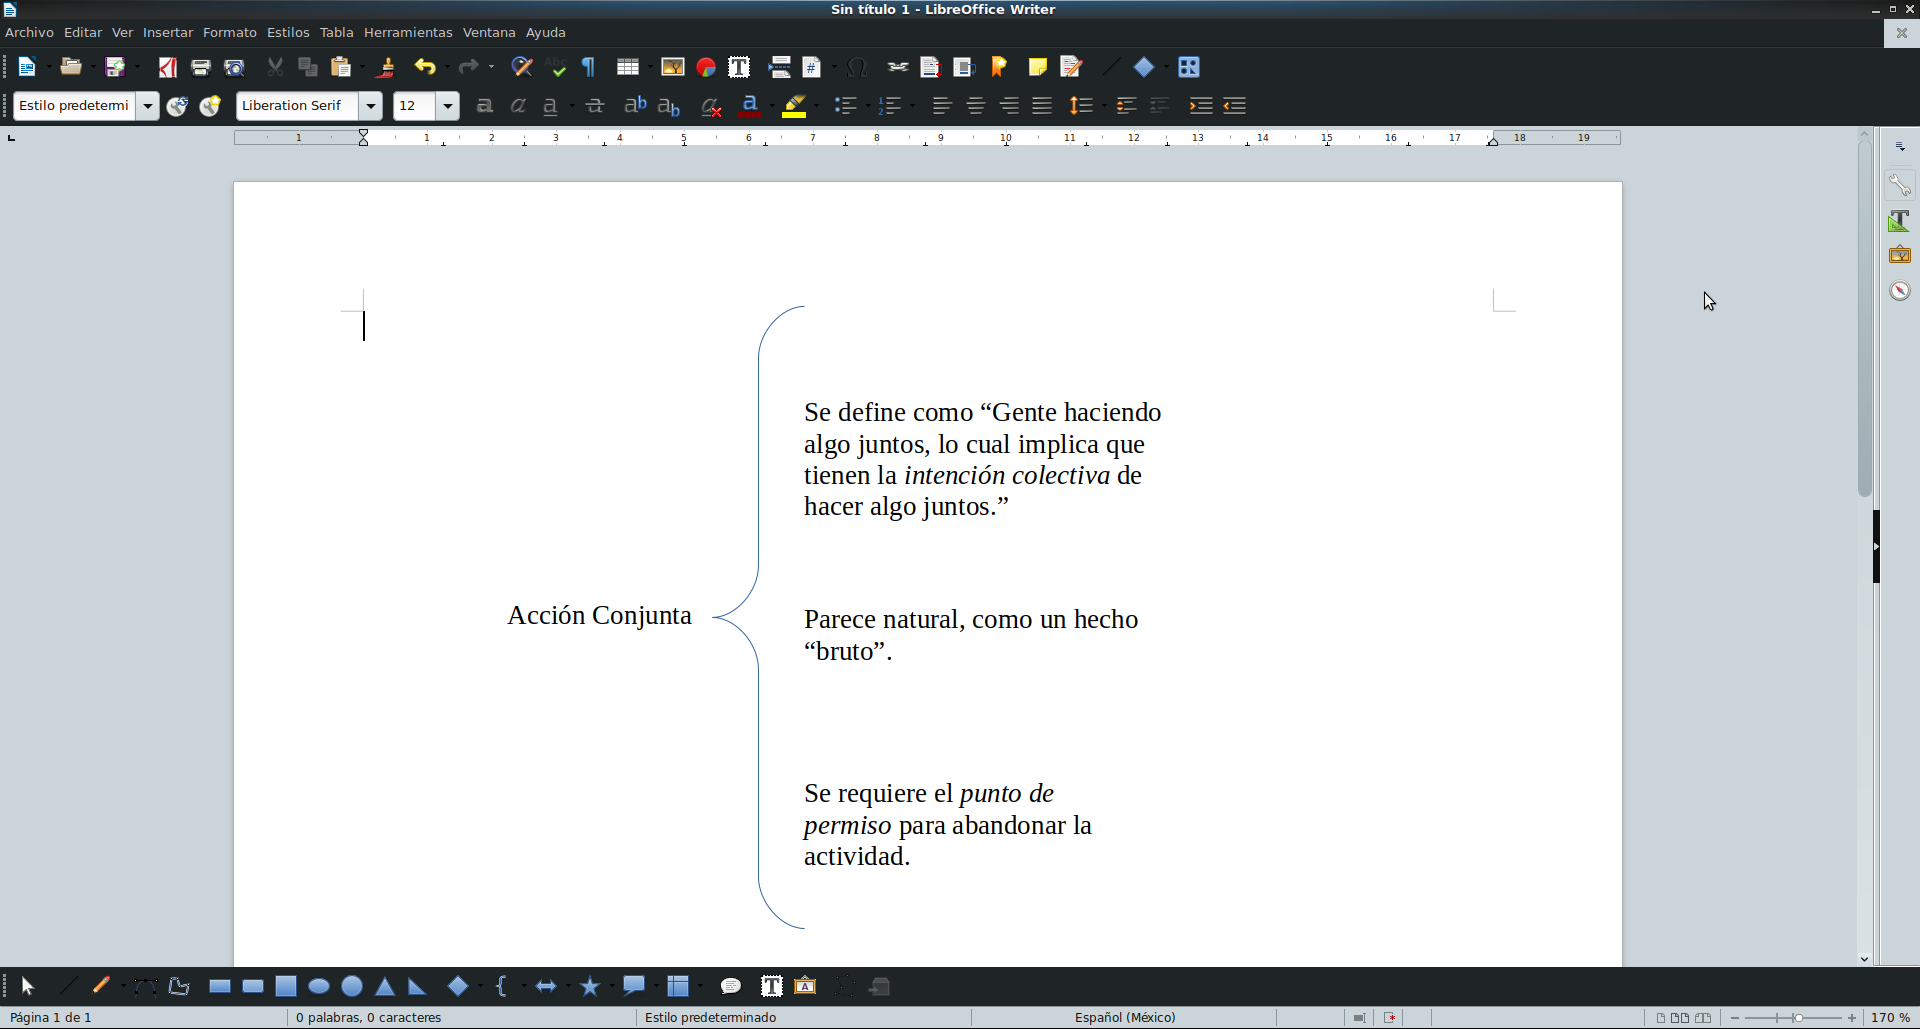
\includegraphics[width=12cm, height=7cm]{img/esquema_4}
	\caption{Acción conjunta}

\end{figure}

\subsection{Compromiso conjunto}
\noindent{Aún nos falta por armar el rompecabezas con las piezas que tenemos y más aun explicar cómo es que el compromiso conjunto es importante para comprender la estructura del átomo social. Y para realizar esto me apoyaré en primer lugar, en la explicación que ofrece el filósofo estadounidense Michael Robins \cite{robins}. Posteriormente examinaré la propuesta de Margaret Gilbert. La explicación del primero, ayudará a tener presente qué es un \textit{compromiso condicional personal} (CPC), el cual retomaré para exponer la propuesta de Margaret Gilbert.}

Michael Robins define un compromiso conjunto como un compromiso de la naturaleza condicional personal, abreviado como CPC, que puede ser interpretado en términos de intenciones personales condicionales, donde cada una de las intenciones ha sido expresada \footnote{Gilbert, Margaret. \textit{The Structure of the Social Atom: Joint Commitment as the Foundation of Human Social Behavior en Socilaizing Methaphysics}. F. S. Schmitt ed. p. 51.}.

Vemos entonces que lo que subyace al Compromiso Personal Condicional son las Intenciones Personales Condicionales. Por lo que si esclarecemos el significado de estas intenciones, llegaremos a la comprensión  del CPC.

Michael Robins explica que las intenciones personales condicionales son de la forma: “yo intento hacer A si y sólo sí, una cierta condición se cumple”. Estas también se han distinguido en dos clases: intenciones personales \textit{internamente condicionales} e intenciones personales \textit{externamente condicionales}. La primera es una expresión de la forma: “Yo intento hacer algo si una cierta condición se cumple”. Y la segunda es del modo: “Si una cierta condición se satisface, yo intento esto”.

En otras palabras, las \textit{intenciones personales condicionales} se pueden entender como proposiciones lógicas bicondicionales ($P \leftrightarrow Q$), en el que la intención personal \textit{internamente condicional} es la implicación lógica  $P \rightarrow Q$; mientras que la intención personal \textit{externamente condicional} es la implicación $Q \rightarrow P$. De este modo, Q es una condición necesaria y suficiente para P.


Este tipo de \textit{intenciones}, más allá de su formalismo lógico, se puede notar que son intenciones personales, y esto significa que está en cada persona la decisión final para realizar cierta acción. Por ejemplo, supongamos que dos personas se comentan: 
\\


\begin{quote}

	\textit{-Hola. Quiero ir a dar un paseo. Si te interesa vamos juntos.}

	\textit{-Sí, sí me gustaría, e iré contigo si tú también quieres.}
\end{quote}

A continuación presento un breve esquema para ilustrar el planteamiento de Michael Robins:

\begin{figure}[h]
	\centering
	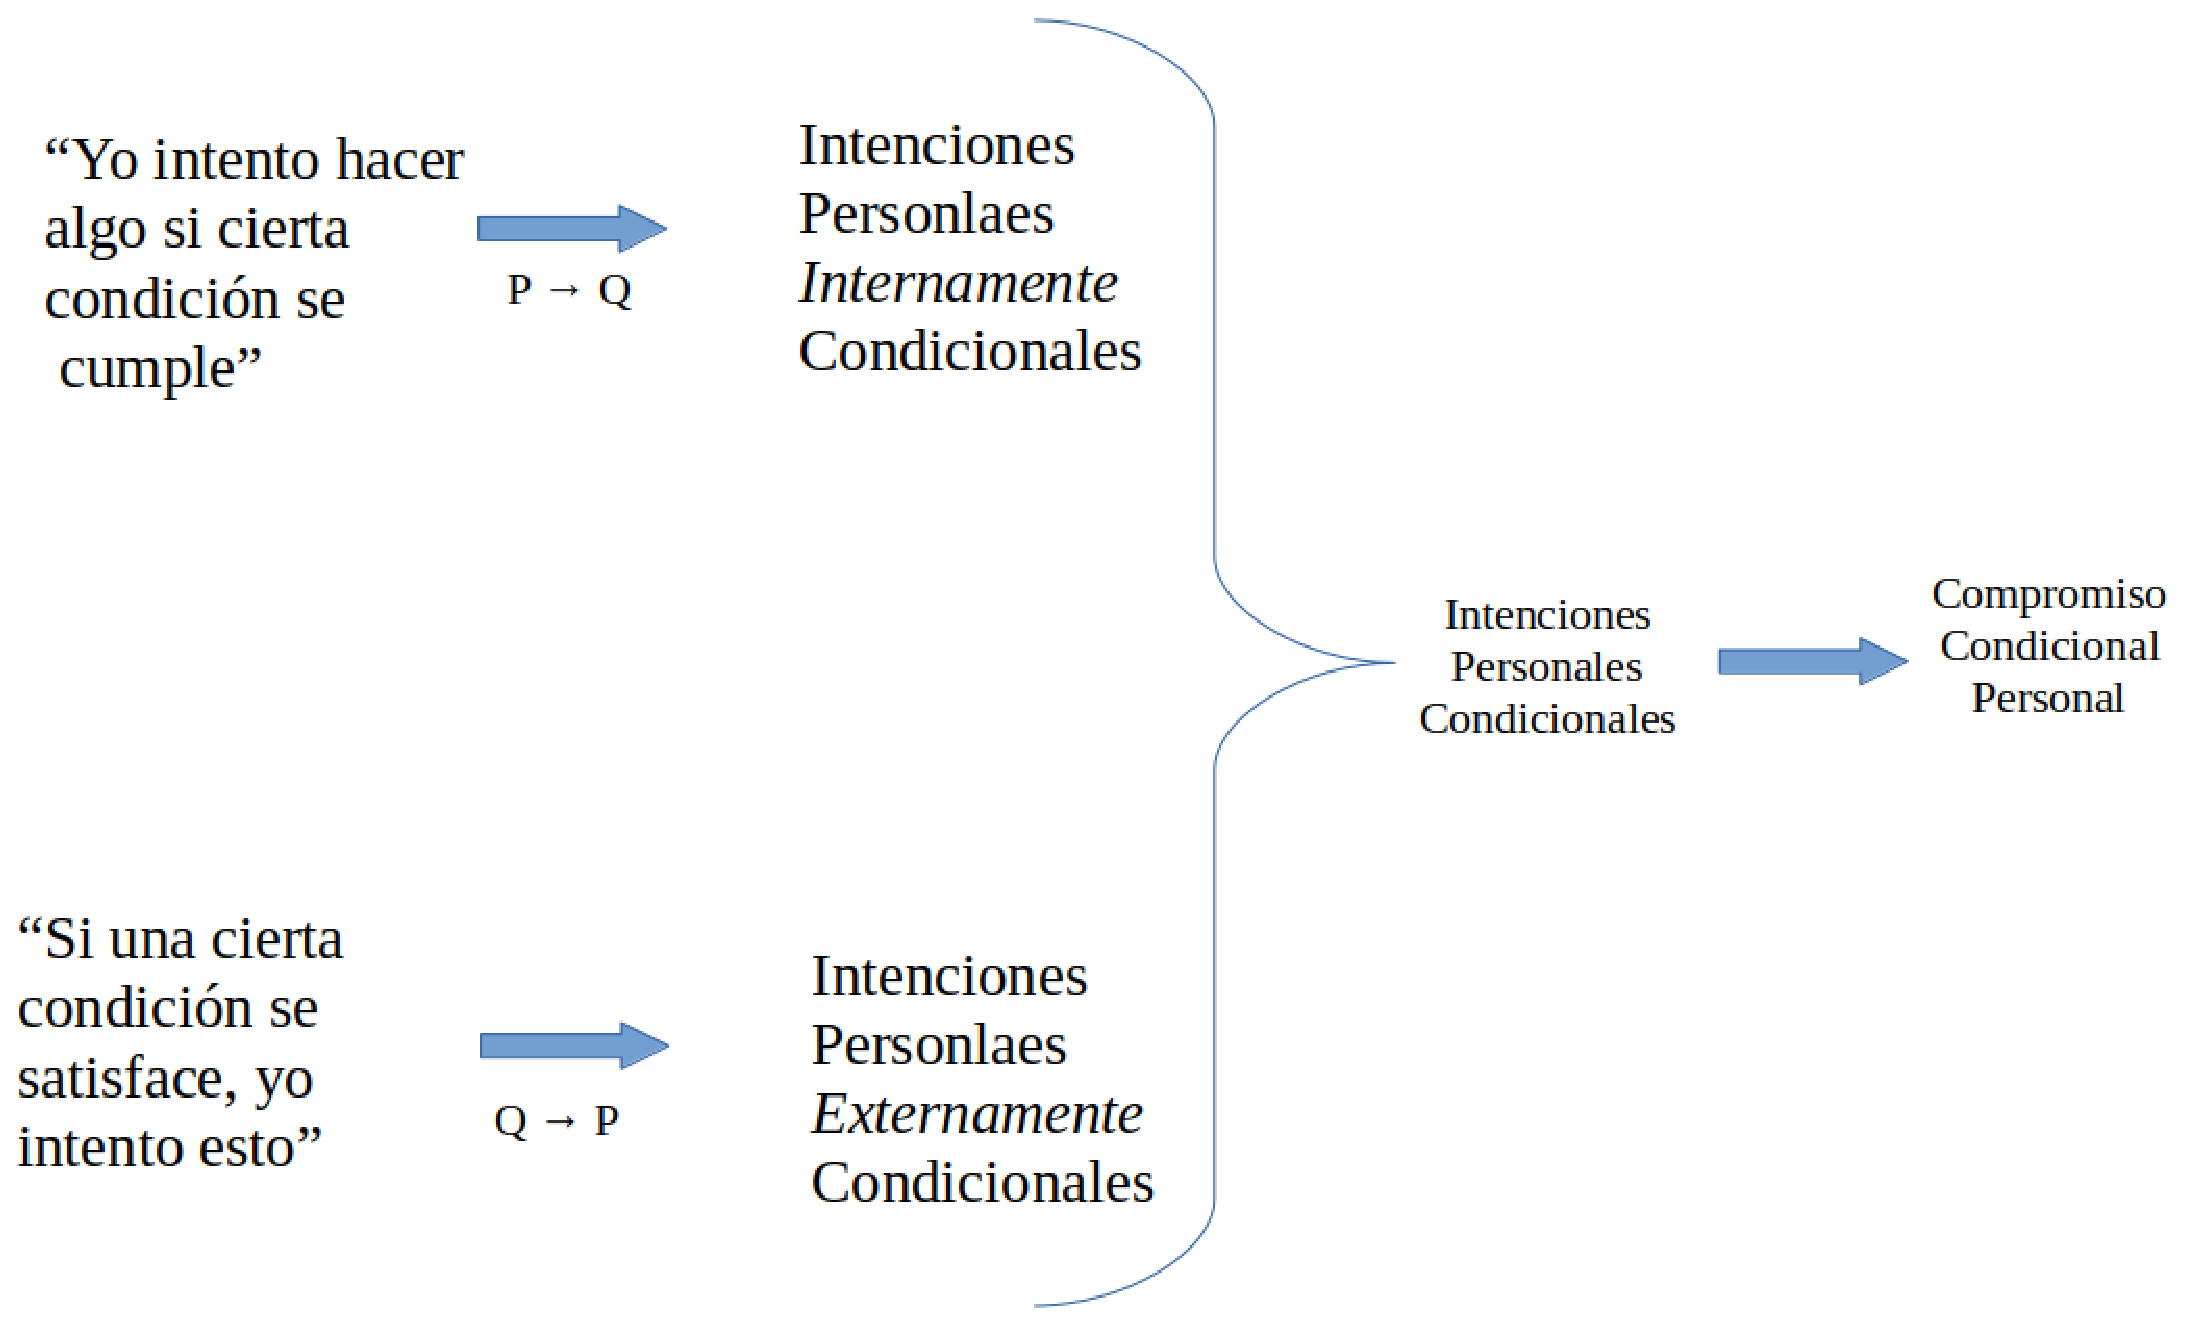
\includegraphics[width=11cm, height=6cm]{img/esquemaRobins}
	\caption{Compromisos Personales Condicionales (CPC)}
\end{figure}


Con lo cual se expresa en cada una de las partes la intención personal de hacer lo necesario para contribuir en llevar a cabo la actividad. La intención de estos dos personajes es una \textit{intención personal condicional.}

Este tipo de compromiso conjunto depende de la \textit{intención personal condicional} de cada individuo que está involucrado, cada una de las intenciones tiene que ser expresada de modo que cada individuo tiene claro quiénes forman parte del compromiso.

Es decir se tiene presente quiénes establecieron el compromiso condicional personal por lo que las participaciones se pueden considerar de manera nominal.

Y al ser así este compromiso se puede definir como la sumatoria de las \textit{intenciones personales condicionales} de los miembros involucrados en el compromiso conjunto.

En resumen. La propuesta de Michael Robins apela a un compromiso conjunto del tipo condicional llamado \textit{Compromiso Condicional Personal} el cual se explica al sumar las \textit{intenciones personales condicionales} expresadas por cada uno de los miembros que participan.

Esta propuesta es interesante y en una primera impresión, se puede pensar en términos de democracia participativa, en el que el compromiso colectivo que se tiene sobre cierta decisión corresponde con la suma de decisiones personales expresadas por medio de una urna. Sin lugar a dudas es una reflexión que hay que tomar en cuenta y que es parte de toda una discusión que hay que seguir teniendo.

Ahora veamos la propuesta de Margaret Gilbert.

Mientras la propuesta de \textit{compromiso conjunto} de Robins es interpretada desde las \textit{intenciones personales condicionales}, y como la suma simple de los compromisos personales; la propuesta de Gilbert, se basa en que las partes expresan su \textit{disponibilidad personal.}
\\

Veamos que significa esto. Empecemos por explicar la noción de \textit{disponibilidad personal.}

A diferencia de Michel Robins Margaret Gilbert en vez de referirse a expresiones de \textit{intención condicional}, se refiere a las de la \textit{voluntad} para estar comprometidos o \textit{disponibilidad} para estar comprometidos conjuntamente.

Para que haya \textit{disponibilidad conjunta} cada uno de lo miembros deben primero expresar su \textit{cuasi-disponibilidad}.	Por ejemplo,  una situación de cuasi-disponibilidad sería el caso de dos sujetos que intentan lograr un objetivo en común, el cual uno le pregunta al otro “¿Estamos listos verdad?”

Es importante tomar en cuenta estas expresiones de voluntad, pues el \textit{compromiso conjunto} se obtiene cuando por lo menos dos expresiones de disponibilidad personal se logran empatar\footnote{\textit{Ibíd}. P. 41.}. Y cuando se llega a este punto, la expresión \textit{cuasi-disponible} alcanza una expresión de \textit{disponibilidad personal} para entonces ser conjuntamente comprometido como un \textit{cuerpo}, o \textit{conjuntamente disponible.}

Así el \textit{compromiso conjunto} se obtiene cuando por lo menos dos expresiones de \textit{disponibilidad personal} son manifiestas.\footnote{\textit{Ibíd.} P. 54.} Y cuando esto ocurre, también se alcanza una expresión para estar conjuntamente comprometidos como un \textit{cuerpo}\footnote{\textit{Vid. Supra}}.
\\

Con esto Margaret Gilbert se desmarca de la propuesta de Michael Robbins, pues no defiende una propuesta basada en intenciones personales condicionales pero sí aboga por una noción de disponibilidad \textit{holista}.

En palabras de Gilbert,

\begin{quotation}
He afirmado que las partes deben abiertamente expresar algo, donde estas expresiones deben de ser de común conocimiento entre las partes. Algo que debe de ser expresado siendo una y la misma cosa para cada uno de los que expresan, mutatis mutandis. 

[...]

Lo que es la clave es la incorporación de una noción holística de compromiso conjunto. La formulación correctamente implica que las partes de algún compromiso conjunto debe de poseer esta noción. También con razón está presente la idea de que, como las partes entienden la existencia del compromiso conjunto relevante, entonces cada uno de ellas está comprometido de manera dependiente a través de los que expresaron la misma cosa, mutatis mutandis\footnote{\textit{Ibíd.} P. 53.}.
\\
\\
\\

\end{quotation}

Ese “algo que debe de ser expresado” para Gilbert no es más que el entendimiento de que, si y sólo si es de conocimiento común que las otras partes relevantes hayan expresado compromisos similares, las partes en cuestión están incondicional y conjuntamente comprometidas.

Este compromiso no está constituido por una serie de compromisos personales, sino que más bien este es de naturaleza holista y por ello debe ser analizado en términos del \textit{todo} y no a través de las partes que lo componen\footnote{Gilbert, Margaret (1989). \textit{On Social Facts}. Londres: Routledge. P. 49}. 

\begin{figure}[h]
	\centering
    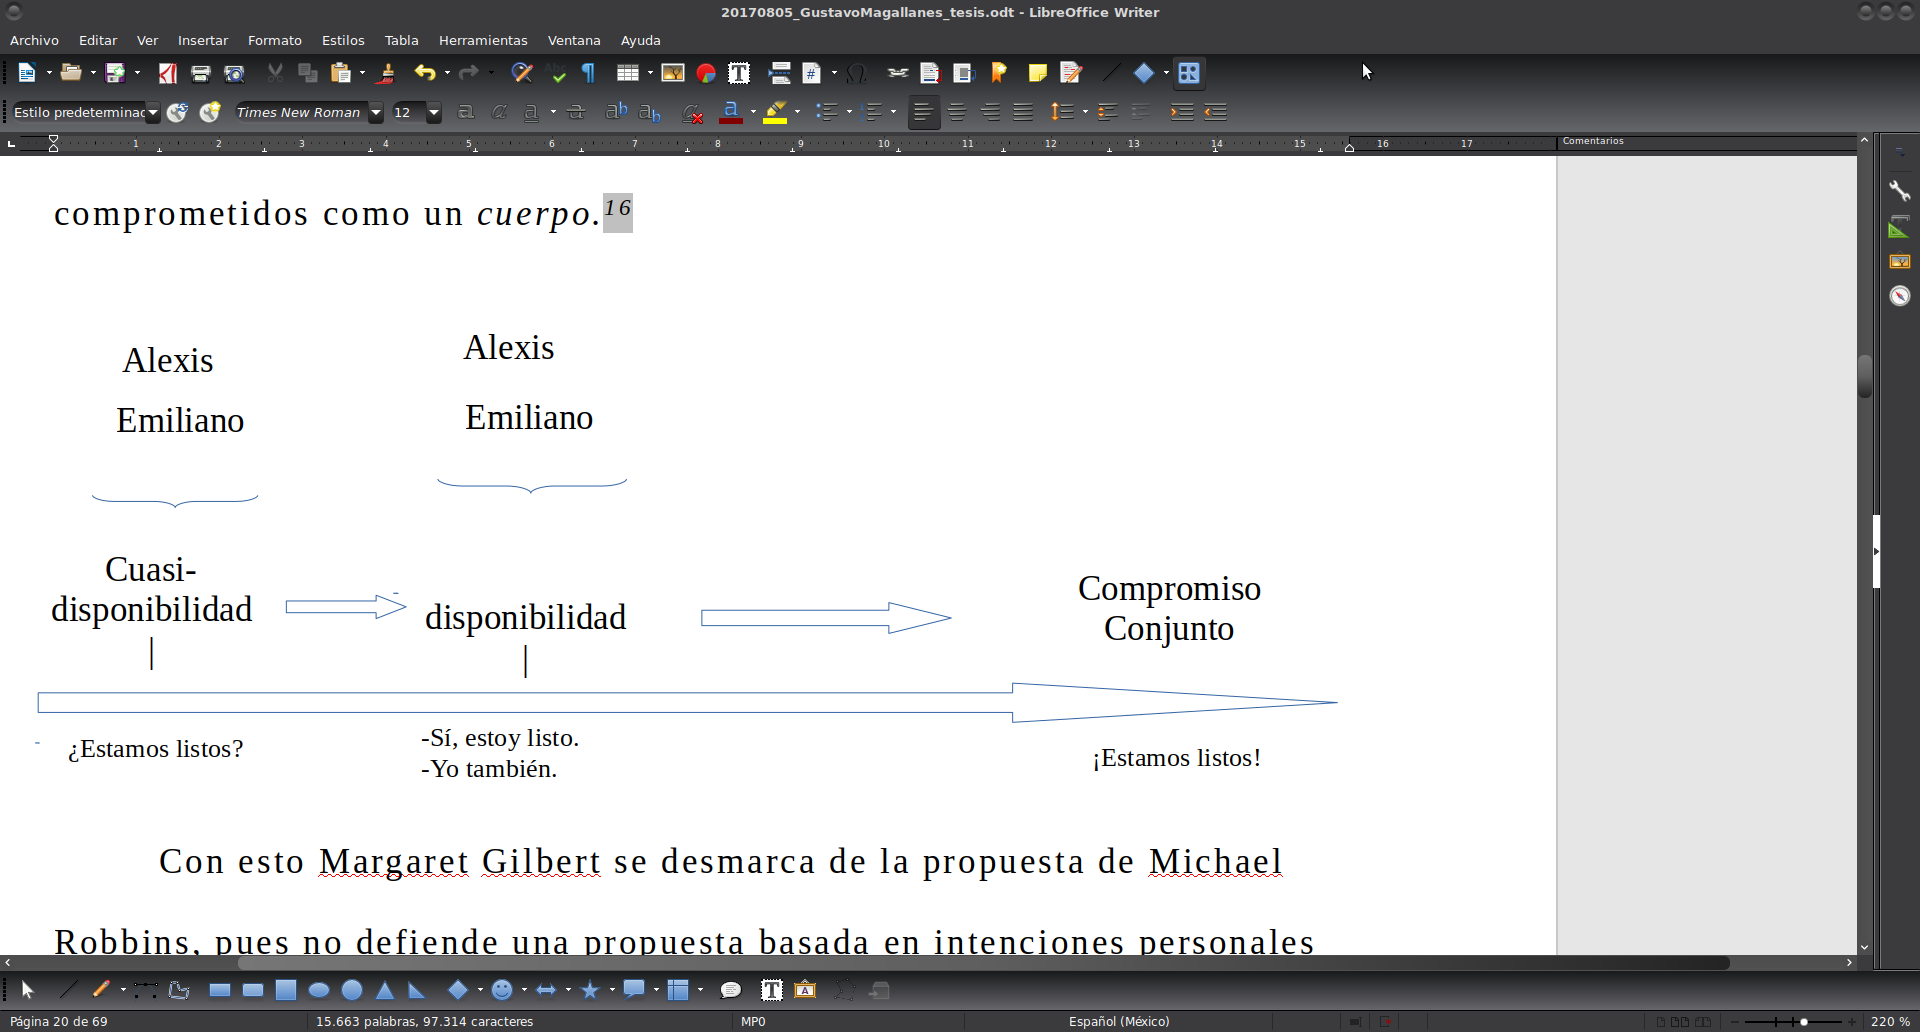
\includegraphics[width=12cm, height=5cm]{img/esquema_2}
	\caption{Disponibilidad para actuar en un \textit{compromiso conjunto.}}
\end{figure}


Es decir, se debe de entender cómo un sistema total, integrado en el que cada parte es responsable frente a todas las demás por alguna violación del compromiso conjunto o de su cumplimiento. 

El tipo de compromiso que defiende Gilbert contiene una serie de características centrales que conviene revisar para tener presente cómo es que se configura este compromiso. En seguida expongo algunas de estas características, que si bien no son todas, presentaré sólo aquellas que son pertinenetes para seguir el desarrollo de esta tesis\footnote{\textit{Ibíd.} P. 49.}:

El \textit{holismo} es una característica importante del compromiso conjunto, pues como se mencionó anteriormente no es una sumatoria de intenciones.

La \textit{responsabilidad}, porque cada parte es responsable hacia todas las demás por alguna violación del compromiso conjunto. Esto es precisamente una función del estar juntos. 

\textit{Derechos y obligaciones}, porque cada parte tiene derechos y obligaciones hacia las partes involucradas. Son obligaciones para actuar de acuerdo al compromiso establecido, y derechos sobre su ejecución. 

La \textit{creación} de un compromiso conjunto requiere la participación de todas las partes. Sin embargo, puede darse el caso de que las partes permitan la creación de compromisos por parte de una persona. Pero de ser así, significaría que dicha persona fue creada también con cierta autoridad unilateral para crear compromisos conjuntos.

Un compromiso conjunto no es rescindible unilateralmente por alguna de las partes, sino por todas las demás en conjunto. Sin embargo, hay que aclarar que existen situaciones en las que entendimientos previos o preliminares explícitos llevarían a la rescisión unilateral. 

Otro atributo que Gilbert señala es el de los \textit{compromisos individuales dependientes}. Esto es que, cuando hay un compromiso conjunto, cada una de las partes está comprometida a través de él. En este sentido, uno puede hablar de “compromisos individuales” asociados de las partes, pero estos compromisos existen a través del mismo compromiso conjunto. Por otro lado, cada uno de los contenidos de los compromisos individuales están (presumiblemente) comprometidos a promover el objeto del compromiso conjunto, por lo que hay dependencia entre los compromisos individuales.

\textit{Compromisos no personales dependientes}. Este atributo nos dice que dada su existencia a través del compromiso conjunto, estos compromisos individuales no son compromisos personales: es decir, no son la creación unilateral de las personas involucradas, no pueden ser unilateralmente rescindidos los compromisos individuales; y uno es responsable hacia todos por alguna violación al compromiso conjunto.

También hay \textit{interdependencia de compromisos dependientes}. Lo que significa que los compromisos individuales dependientes son interdependientes en el sentido de que no puede haber un compromiso singular de esta naturaleza perteneciente a un determinado individuo, en ausencia de algún otro compromiso.
\\
\\

\textit{Simultaneidad de compromisos dependientes}. Los compromisos individuales dependientes de las partes nacen simultáneamente al de la creación del compromiso conjunto.

\textit{Contenido}. Los compromisos conjuntos son compromisos para actuar como un cuerpo de una forma específica. Esto significa que: La gente puede comprometerse conjuntamente a \textit{aceptar}, \textit{intentar}, \textit{creer} como un cuerpo. Y por otro lado, las partes están conjuntamente comprometidas para constituir tan lejos como es posible, un solo cuerpo para actuar en el modo en cuestión. Por ejemplo: Ellos están comprometidos conjuntamente para constituir tan lejos como es posible, un solo cuerpo para aceptar algo como objetivo propio \footnote{Para explicar con más detalle el texto Gilbert, Margaret. (2003). \textit{The Structure of the Social Atom: Joint Commitment as the Foundation of Human Social Behavior} en Socilaizing Methaphysics. F. S. Schmitt.}.

Todas estos atributos caracterizan la noción de compromiso conjunto, pero como señalé anteriormente no son todas y todavía se puede seguir explorando al respecto.

\begin{figure}[h]
	\centering
	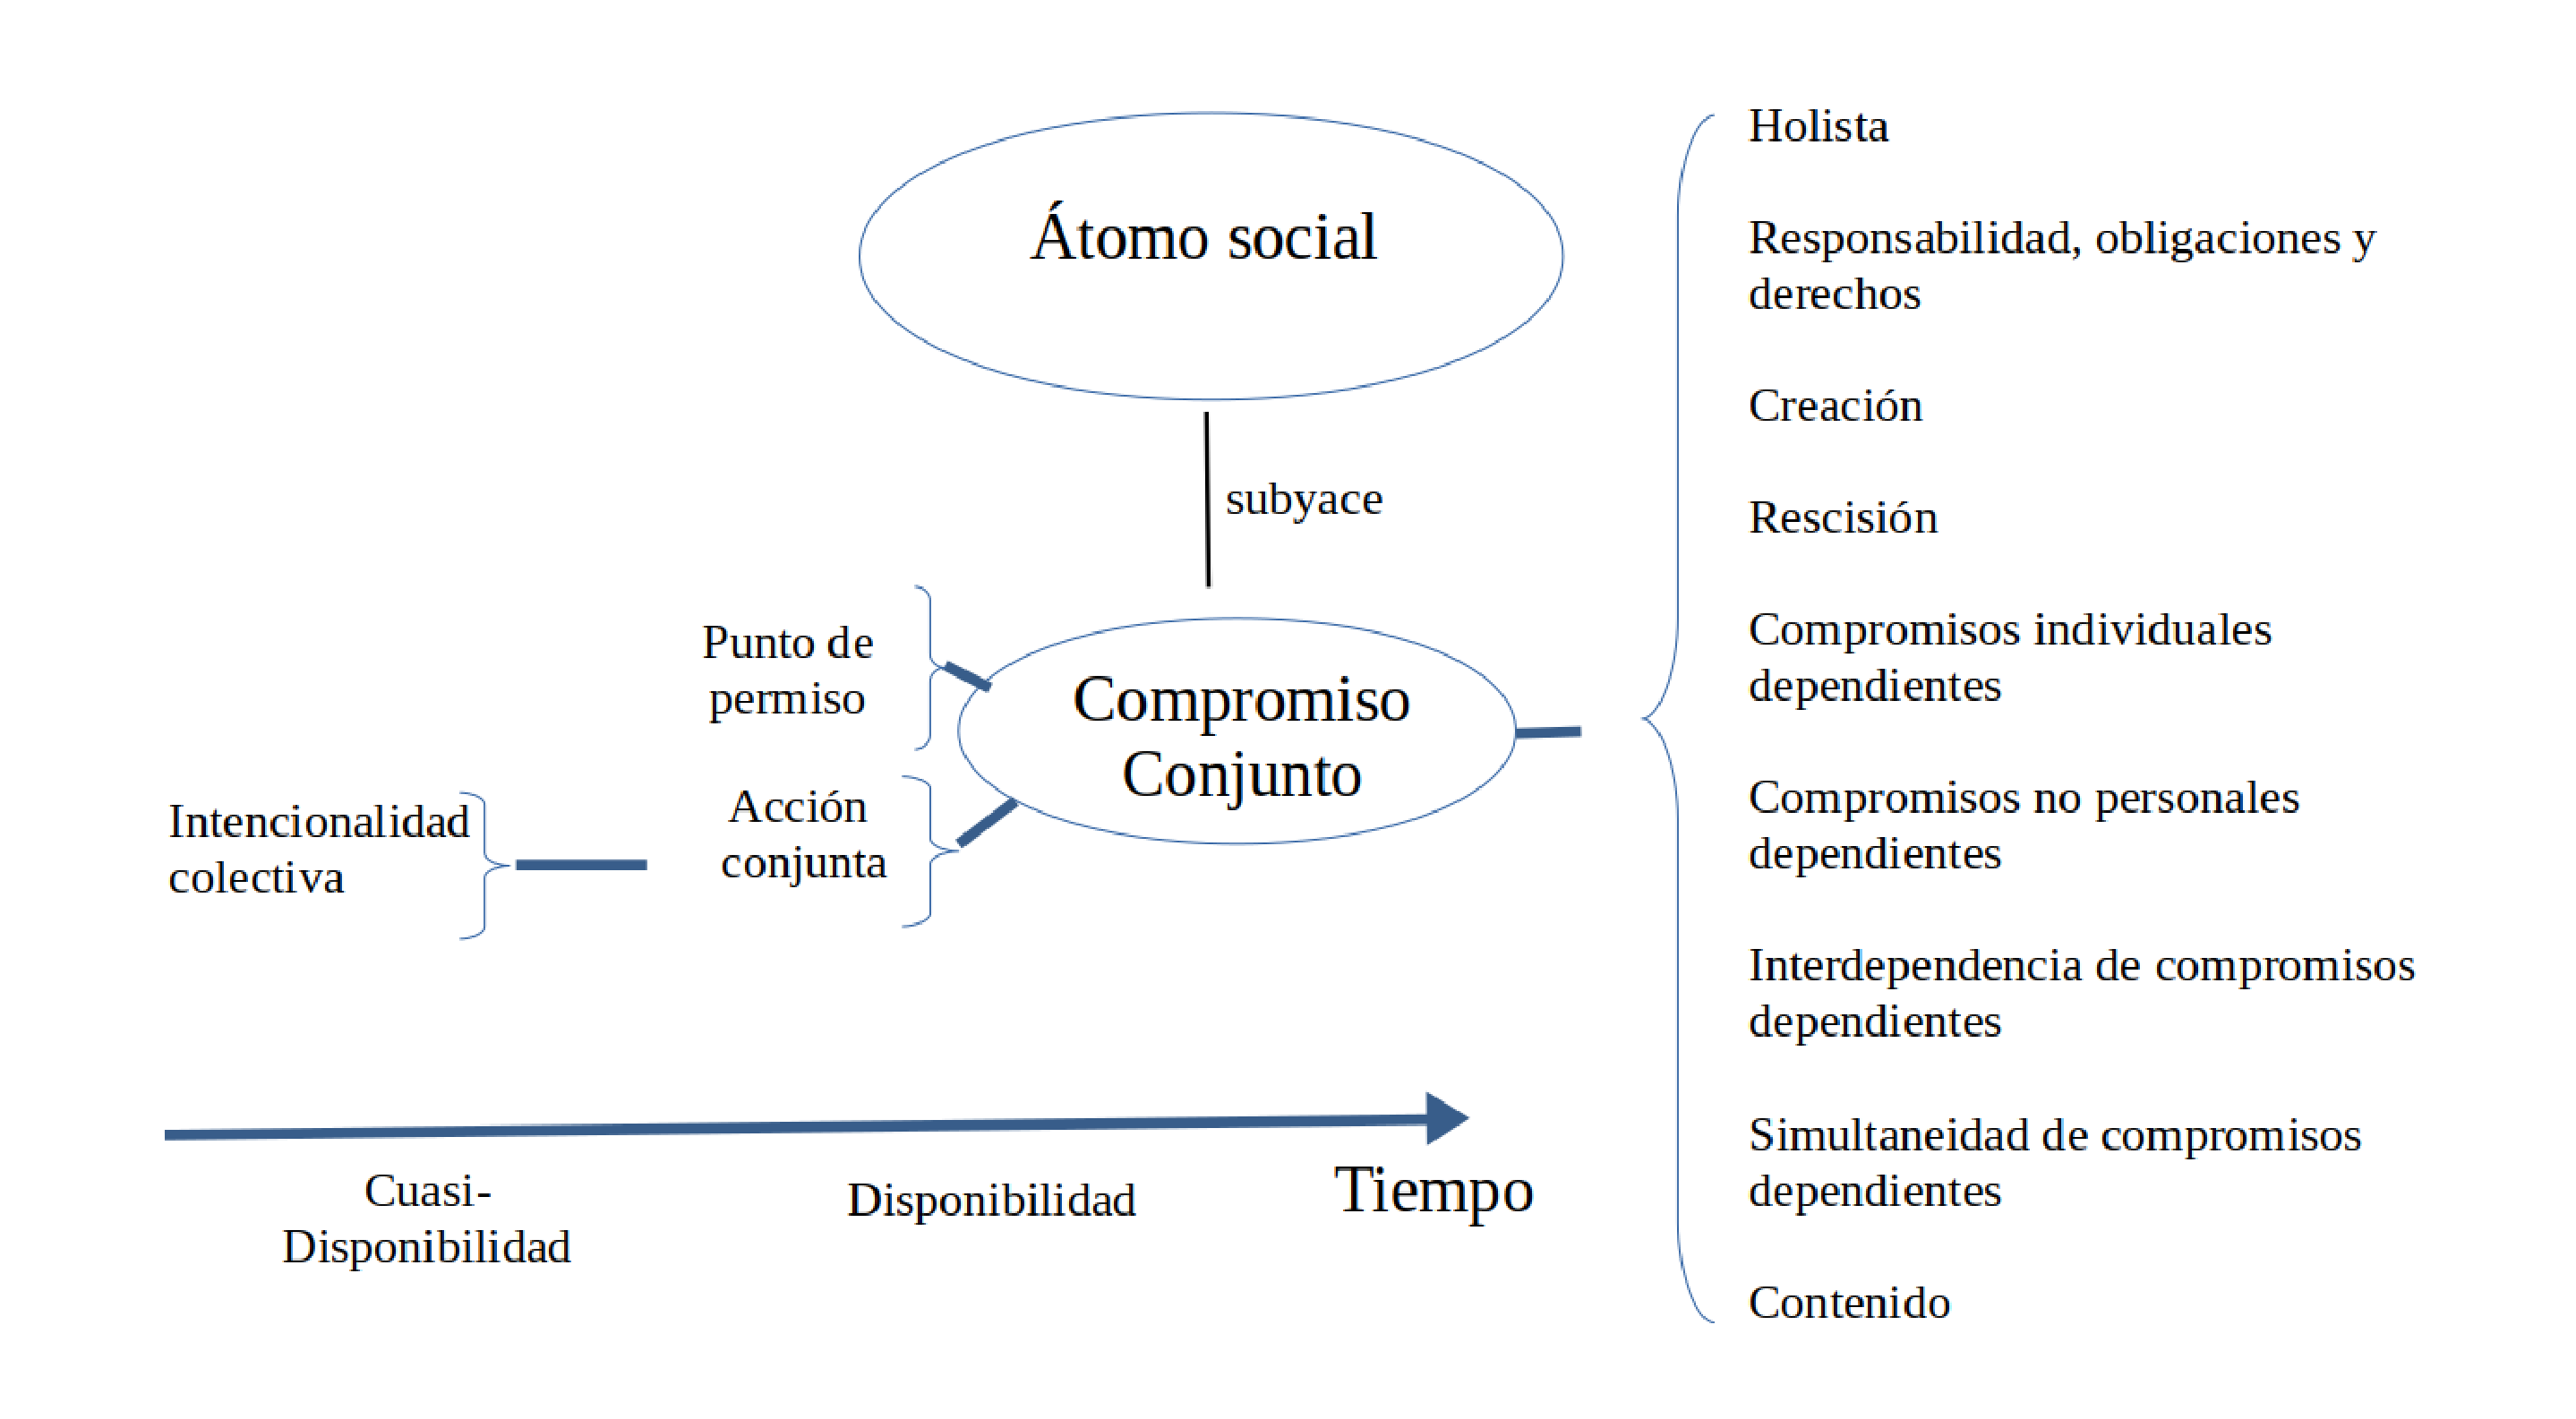
\includegraphics[width=12.5cm, height=8cm]{img/esquema_3}
	\caption{Estructura del Átomo Social.}
\end{figure}

Con lo expuesto, ya tenemos un acercamiento a la noción de compromiso conjunto de Margarte Gilbert. Y se puede pensar ya no como un átomo sino como una entidad sujeta. Esto nos conducirá a establecer una noción de Nosotros que nos permitirá avanzar en este trabajo.

\section{Átomos sociales, sujetos plurales y compromiso conjunto}

\noindent{Para Margaret Gilbert, un \textit{sujeto plural} es cualquier grupo de personas conjuntamente comprometidas\footnote{Gilbert, Margaret. (2003). \textit{The Structure of the Social Atom: Joint Commitment as the Foundation of Human Social Behavior} en Socilaizing Methaphysics. F. S. Schmitt ed. P. 55.} como podrían ser: familias, sindicatos, gremios, etc., los cuales pueden ser regidos por reglas, convenciones, acuerdos cotidianos, creencias colectivas, valores. Y pueden ser pequeños y fugaces, o bien, grandes y relativamente permanentes.}

De esta manera, el átomo social es un sujeto plural pero en su unidad social mínima. Por lo que es fundamental comprender la estructura del compromiso conjunto para entender la noción de \textit{átomo social}, y por ende la del \textit{sujeto plural}.

Esta noción de \textit{Sujeto Plural}, entendida también como \textit{Nosotros} resulta ser interesante para entender como es que se configuran las relaciones sociales en términos de compromiso, trabajo, e intenciones en las colectividades. En la filosofía contemporánea, por ejemplo, la noción de \textit{sujeto plural} ha sido abordada desde varios autores. Uno de ellos es el del filósofo irlandés Phillip Pettit\cite{pettit}, quien sostiene que las colectividades integradas, no sólo operan en el mismo sentido que las personas individuales, sino que también tienen la capacidad de pensar en términos de primera persona. Es decir, que en una colectividad las palabras sobre “nosotros”, se destacan como las palabras que unen y comprometen a la colectividad como un \textit{sujeto plural}.

Pero también esta noción de Nosotros se puede pensar ya no sólo desde el enfoque en el que se considera únicamente a las personas como parte del colectivo, sino en un sentido mucho más amplio en el que los integrantes comparten el entorno social, político y natural. Por lo cual se considera a las plantas, los animales, los bosques, y las montañas como parte de ese Nosotros. 
\\
\\

Me refiero al tipo de nosotros que describe Carlos Lenkersdorf y el cual nos interesa abordar para trazar, junto con el Sujeto Plural de Gilbert, el Nosotros de los pueblos zapatistas.

Para esta tarea considero que no únicamente con las ideas de Carlos Lenkersdorf podré aproximarme a este Nosotros de los pueblos zapatistas, sino que además necesitaré apoyarme en el concepto de \textit{comunitarismo} que desarrolla Luis Villoro para poder tener un Nosotros un poco más completo.

\chapter{El Nosotros de los pueblos zapatistas}
\noindent{El haber revisado cómo es que se pueden estudiar y comprender las entidades colectivas desde el examen de las oraciones me proporcionó soporte para realizar este mismo ejercicio pero sobre las palabras escritas y expuestas en distintos momentos por los pueblos zapatistas.}

Y es bajo este examen, en el cual señalo que el Nosotros de los pueblos zapatistas se puede proponer desde por lo menos tres elementos: La palabra, el acuerdo y el trabajo colectivo.
\\

Propongo a la \textit{palabra} porque, como expondré con más detalle, contiene un significado al que los pueblos le dan un cierto peso de compromiso que no se puede soslayar. No es el simplemente mencionar algo, sino que también se acarrea en ésta cierta importancia que hay que atender. Además este tipo de palabra incluye no sólo a personas sino también al entorno natural.

El \textit{acuerdo} es otro de los elementos que tomo en cuenta en la conformación de esta entidad colectiva. Pues considero que es precisamente en este punto en el que se cohesiona el grupo y se formula un Nosotros. Y es aquí en dónde me es pertinente el análisis de Margaret Gilbert, ya que esto se puede entender también desde la óptica del compromiso conjunto.    

También el \textit{trabajo colectivo} es un elemento importante en el que este Nosotros no se vuelve algo efímero, sino con un tiempo de vida prolongado y que lo mantiene con cierta vitalidad.

Finalmente la \textit{Comunidad} es esa entidad en la que la \textit{palabra}, el \textit{acuerdo}, el \textit{trabajo colectivo} y el \textit{Nosotros} están presentes. Es la entidad que puede contener desde un Nosotros y varios a la vez.

A continuación expongo cada uno de estos elementos. 

\section{La Palabra}
\noindent{Son múltiples los comunicados y escritos del EZLN en los que se menciona la \textit{palabra} como un elemento que está presente en sus relaciones sociales. Y haciendo un examen de lo que ésta significa para quienes la mencionan así como para quienes la escuchan en estos pueblos resulta revelador la importancia que la palabra tiene para el grupo o colectivo. }

Ejemplo de esto lo vemos en el mensaje de bienvenida a la Segunda Reunión Preparatoria de la Sexta en territorio de la Junta de Buen Gobierno de La Garrucha, en la comunidad zapatista de Carmen Pataté, el 13 de agosto de 2005\footnote{En línea en << http://enlacezapatista.ezln.org.mx/2005/08/13/2a-reunion-preparatoria-palabras-de-inicio/ >>.}. Que aunque es un poco largo el extracto de la historia que presento, ruego al lector su comprensión pues me parece que esclarece la importancia y el peso al que me refiero. 

En esa ocasión se dijo:

\begin{quote}
Les quiero contar una historia. Como esta es la reunión de pueblos indios y organizaciones indígenas, pues vamos a tratar de hablar así como es nuestro modo pues, entre indígenas, entre pueblos indios. Y un poco es la historia que cuentan nuestros antepasados mayas, de cómo empezó todo el mundo. Entonces dicen pues, que cuentan nuestros antiguos, que al principio no hay nada y en realidad el mundo se empieza a andar, echa a andar cuando aparece la palabra. Pero no nada más que la palabra aparece así, sino que la palabra, dicen los antiguos, empieza a pensarse a sí misma para dentro, dicen, a reflexionar. Por medio de la palabra los primeros dioses, los que forman el mundo se empiezan a consultar entre sí, se hablan, se ponen de acuerdo y se reflexionan. Y entonces, ya que hacen acuerdo se juntan, juntan su pensamiento y entonces es cuando se echa a andar el mundo. Así empezó todo, con la palabra que se piensa para dentro, o sea, que se reflexiona en el corazón que es espejo para dentro para mirarnos lo que somos. Y ya luego pues fue la palabra que se encuentra con otra palabra. No peleaba la primera palabra, no quiere dominar, no quiere vencer a la otra palabra y es porque la primera palabra que sale, encuentra una palabra que es como su hermana, porque es igual aunque es diferente. O sea, que como que tiene la misma raíz, pero es rama o es hoja del árbol del mundo. O sea, que la primera palabra no estaba sola, sino que había otra palabra y según este pensamiento que es el de nuestros antiguos mayas, el mundo empieza a nacer cuando esa una palabra y esa otra palabra se encuentran y no hacen pleito sino que se encuentran y sacan acuerdo porque se respetan mutuamente entre ambas y se hablan y se escuchan.
\end{quote}

Esta historia nos proporciona algunas pistas para comenzar a realizar el análisis. Por ejemplo en la oración se menciona que con la palabra se piensa, se reflexiona con el corazón. Lo cual nos indica que ésta encierra cierta importancia que le da quien la escucha. Y que la tiene presente no sólo en su reflexión sino en algo más que rebasa el pensamiento.

También se señala que la palabra que ellos expresan, no quiere dominar, ni vencer a la de los demás y es porque se entiende que las palabras son importantes e iguales y diferentes también para todos. Con esto se busca algún tipo de acuerdo en el que se no se imponga una opinión sobre las demás. Sino que se busca generar algún tipo de consenso. Algo que es difícil de lograr si no se tiene la intención de escuchar la palabra del otro y hacerla propia también.

Y en el diálogo no se agreden sino que se encuentran y sacan acuerdos porque se respetan mutuamente entre ambas y se hablan y se escuchan. Con lo que se puede apreciar que se busca privilegiar el diálogo escuchando y atendiendo las palabras del grupo.

La noción de \textit{palabra} que me interesa abordar es precisamente aquella que se escucha, se atiende, se comparte y se “piensa con el corazón”. Es un poco difícil de explicar cómo es que se realiza esto en este momento, pero con la noción de intersubjetividad de Carlos Lenkersdorf quedará esto más claro.

\subsection{La palabra y la noción de intersubjetividad de Carlos Lenkersdorf}
\noindent{Carlos Lenkersdorf fue un filósofo y lingüista mexicano de origen alemán que dedicó años de su vida al estudio y reflexión sobre la noción de Nosotros\footnote{No está de más decir que realizó sus investigaciones en zona tojolabal en el sureste mexicano y publicó varios libros al respecto. Además dirigió durante años un seminario en la Facultad de Filosofía y Letras de la UNAM precisamente sobre el concepto de Nosotros.}}

Es por este motivo es que considero que las ideas de Carlos Lenkersdorf pueden ayudarme a comprender cómo se conforma la noción de Nosotros en los pueblos zapatistas, pues su metodología se centra en el análisis de las palabras que enuncian los tojolabales buscando siempre cómo es que se genera y conforma una entidad colectiva nosótrica. 

En este sentido uno de los conceptos que me interesa abordar del trabajo de este autor es la noción de \textit{intersubjetividad}.

Y en principio lo que nos dice el autor sobre el significado de este concepto es que es aquella relación que se da entre sujetos-sujetos. Y en la que todos son sujetos aunque de diferentes clases.\footnote{Lenkersdorf , Carlos (2008). \textit{Los hombres Verdaderos. Voces y testimonios tojolabales}. Siglo XXI Editores. p. 46}

Es decir, en las palabras de los pueblos tojolabales se hace mención de todo aquello que conforma su entorno como si fuera un sujeto y no un  objeto. Todo es considerado sujetos. Y más bien lo que hay son sujetos de distintas clases. Un humano y una planta son sujetos, pero de clases diferentes.

En una conversación, por ejemplo, los dialogantes de un grupo se perciben como semejantes y el respeto que algunos de los miembros le da a la palabra es entendida así por los demás. Un árbol, la tierra, las nubes, el agua, los animales, etc., no son considerados en estos pueblos como objetos, sino como sujetos. Todos y cada uno son sujetos.

También bajo este mismo concepto el filósofo nos dice que bajo la intersubjetividad todos son iguales; por ello, se excluye la subordinación de los objetos-mandados a los sujetos-mandones\footnote{\textit{Ibídem.} P. 46}. Como la relación en el diálogo es entre semejantes, se excluye la subordinación entre sujetos. 

El filósofo nos dice que hay en la intersubjetividad una relación entre la necesidad de las personas y los acontecimientos. Es decir, todos se necesitan los unos a los otros para que los acontecimientos se hagan realidad\footnote{\textit{Ibídem.} P. 46}. Acontecimientos que van desde una caminata, ir a chapolear la milpa, pizcar frijol o celebrar una asamblea, en los cuales se requiere de la participación de todos. Todos están presentes en el pensamiento de estos pueblos y todos se necesitan. Y esto permite formar un cuerpo en el que los implicados establecen compromisos, acuerdos y convenios.

Otra característica sustancial de este concepto es que prevalece el respeto entre la comunidad y el mundo, pues todos deben respetarse mutuamente si no quieren destruir la comunidad de todos y el acontecer del mundo\footnote{\textit{Ibídem.} P. 46}. Si un conjunto de personas no respeta a los demás, se daña la relación entre las partes y a la comunidad. Esto puede llegar a afectarla y destruirla. De igual manera, esta falta de respeto se podría dar no sólo entre las personas, sino incluso de una persona hacía una(s) de las parte(s) de la “naturaleza”, puesto que ésta es sujeto también.

Es por ello, que Carlos Lenkersdorf señala en su libro \textit{Los hombres verdaderos}, que en los pueblos tojolabales\footnote{\textit{Ibíd.} P. 83}, cuando las personas se comunican entre sí y con su entorno existe cierto respeto entre los involucrados, no hay subordinación, ni verticalidad, lo que hay es reciprocidad e igualdad\footnote{Carlos Lenkersdorf cuenta que cuando pidió a algunos tojolabales si le podían enseñar la lengua, no respondieron ni sí ni no, sino que dijeron: “tenemos que platicarlo con nuestra comunidad”, palabra sustituta de nosotros. Esa respuesta, según cuenta, “fue su segundo encuentro con el nosotros que ya había percibido en la zona tzeltal. Por un lado es comunitario y, por otro, tiene un impacto profundo en el comportamiento de cada uno de sus componentes. Éstos no responden individualmente; sus respuestas reflejan el pensar y el modo de ser de la comunidad” (\textit{El mundo de nosotros}, entrevista de Ana Esther Ceceña a Carlos Lenkersdorf).}. Y agrega que:

\begin{quote}
el acontecimiento de comunicación en tojolabal los dos sujetos con sus acciones correspondientes no subordinan a nadie, sino que tienen que complementarse. La estructura, pues, no es vertical sino horizontal. Las acciones son bidireccionales entre los dos sujetos. Desde la perspectiva tojolabal, pues, la comunicación es un acontecimiento entre iguales.
\end{quote}

Por lo que en las formas y modos de convivencia de los pueblos tojolabales, la \textit{intersubjetividad} es un factor presente en el devenir cotidiano lo cual es importante considerar para la comprensión del pensamiento de este autor.

Y es en este contexto intersubjetivo dónde la \textit{palabra} que forma el nosotros de los pueblos zapatistas se ubica, y al estar insertada en este contexto es que la palabra funciona con los atributos de la intersubjetividad. 

\section{El Acuerdo}
\noindent{La \textit{palabra} al situarse en un contexto intersubjetivo permite que las partes formalicen compromisos, \textit{acuerdos}. Siendo así, ¿cómo es que se logran estos acuerdos en las comunidades zapatistas?}

Por lo menos son visibles tres vías en que se generan dichos acuerdos: el \textit{consenso}, la \textit{consulta}, y la \textit{votación}.

\subsection{Consenso}
\noindent{Según Carlos Lenkersdorf, en los pueblos tojolabales el acuerdo por consenso se construye de la siguiente forma durante una asamblea:}
\begin{quote}
Mucho se habló. Muchas ideas y opiniones se propusieron y se retiraron. Las voces no afinadas disminuyen y se acercan a una gran calma. Evidentemente, ya no hay ideas variadas ni opiniones encontradas. Las diferencias no afinadas se han terminado. [...] Se levanta la voz de alguien, por lo general de un anciano, de todos modos de una persona que “ya tiene corazón” por su experiencia y sabiduría para captar el sentir, opinar, hablar y callar de los asambleístas. [...] Este es el consenso logrado en el cual todos se saben representados\footnote{\textit{Ibídem}. P. 83}.
\end{quote}	

Generar consenso no es un proceso que se siga de manera automática. Este proceso tiene sus dificultades y sus problemas. Este es un proceso en el que participan los integrantes de la asamblea y su \textit{palabra} es escuchada y tomada en cuenta.

El tema del consenso es un tema de amplio interés para la filosofía. Luis Villoro ha pensado y reflexionado al respecto en sus libros \textit{Creer, saber, conocer}\cite{vill}, \textit{De la libertad a la comunidad}\cite{vi} y \textit{El poder y el valor. Fundamentos de una ética política}\cite{vil}, entre otros.

También analiza este concepto pero desde la perspectiva de las ideas del filósofo africano Kwasi Wiredu:
\begin{quote}
en muchas comunidades indígenas persiste el ideal del consenso, al que se llega por la participación de todo el pueblo en asambleas. La asamblea designa también, para cargos dirigentes, a personas que destaquen por su edad avanzada y su sabiduría. Los gobernantes están sujetos al control de los miembros de la comunidad, como proclama un lema común: deben “\textit{servir obedeciendo}”. Estos procedimientos intentan preservar las relaciones de comunidad; por ello chocan a menudo con el régimen de partidos políticos que la dividen\footnote{Villoro, Luis. Sobre democracia consensual. En torno a ideas de de Kwasi Wiredu en ``La ética del consenso de Kwasi Wiredu. Un modelo africano''. En línea <<http://them.polylog.org/2/fvl-es.htm>> última revisión [9 de agosto de 2017.]}.
\end{quote}

Este consenso se logra con la participación y el consentimiento de los miembros de la comunidad. De esta manera, se toman acuerdos que conciernen al colectivo, tal como es la designación de autoridades, las cuales están al servicio de la comunidad y no al revés, pues son servidores de la comunidad, más no funcionarios.

Asimismo, generar un consenso implica por un lado la participación de las partes involucradas, y por el otro, mantener y ejercer el poder comunitario. En el consenso, las partes se entrelazan en el entendido del servicio comunitario, así como en la construcción de la autonomía.

Para los pueblos zapatistas, el consenso como toma de decisiones es importante, pues la \textit{palabra} no se impone de manera unilateral, tampoco intenta convencer o forzar a las partes, tal como dice su quinto y sexto principio del mandar obedeciendo: “Proponer y no imponer” y “Convencer y no vencer”, más bien se intenta construir un acuerdo en armonía.%, en el que todas las voces son tomadas en cuenta.

Así lo explica el Subcomandante Insurgente Moisés el 3 de enero de 2007 en la participación en la Mesa Redonda “Construyendo Contrapoderes”\footnote{Participación del EZLN en la Mesa Redonda “Construyendo Contrapoderes”, 3 de enero del 2007. El línea en <<http://enlacezapatista.ezln.org.mx/2007/01/04/cuento-para-ninas-de-uno-a-100-anos-nos-reservamos-el-derecho-de-admision/>>}:
\begin{quote}
Y los compañeros y las compañeras que están en la asamblea como ésta —hágase de cuenta que son autoridades pues aquí—, entonces lo que pasa ahí es, entonces dicen: aquí en esto no vamos a dar acuerdo, vamos a ir a discutir, luego vamos a volvernos a reunir, y aquí vamos a proponer cuáles son las propuestas. Y de ahí vamos a hacer un consenso acá, cuáles son las ideas mejores que vemos acá, la que tiene ventaja, y cuál es la que tiene desventaja. Y vayamos a explicar otra vez a nuestros pueblos.
\end{quote}

Es así que en estos consensos, la pluralidad de ideas y opiniones no sólo implica tomar en cuenta la diferencia de los sujetos, sino que conduce a buscar las opiniones de quienes forman el colectivo, las comunidades. Hay un proceso de búsqueda de la palabra, de las opiniones para generar el consenso.

\subsection{Consulta}
\noindent{La consulta es otra de las formas en que los pueblos zapatistas generan un acuerdo. Por ejemplo, en la construcción, difusión y reflexión de la Sexta Declaración de la Selva Lacandona las iniciativas políticas, “primero se consultó con los pueblos, luego con los comités, con los regionales, con los locales y con las bases de apoyo, y ya cuando éstas se hacieron públicas es que estuvieron de acuerdo todos los pueblos”\footnote{\textit{Como se hacen los trabajos} en Revista Rebeldía num. 76. Parte I. Pág. 7.}. }
	
Las consultas que han realizado los pueblos zapatistas, permiten también al colectivo definir con firmeza sus pasos hacia adelante. Así por ejemplo, un año después del alzamiento, las comunidades zapatistas convocaron a una consulta nacional e internacional para trazar su camino político. Los zapatistas dijeron en aquel entonces: “Nos estamos dirigiendo a todos nuestros hermanos para proponerles una consulta nacional e internacional que nos oriente a todos sobre los pasos que debemos dar y el rumbo que debemos seguir en este momento histórico”\footnote{Comunicado del Ejército Zapatista de Liberación Nacional: Convocatoria a la Consulta Nacional (1995).}.

En la consulta, los participantes son tomados en cuenta sin importar el espacio ni el tiempo, es decir, se puede aplicar en geografías diversas, y respetando la disponibilidad de calendario de las partes. Las decisiones sólo se hacen públicas cuando todos están de acuerdo, es decir, cuando existe un consenso.

Este \textit{acuerdo} ayuda a que la comunidad en su conjunto crezca y se fortalezca a partir de la coordinación de responsabilidades entre sus miembros. Así lo expone Fanny, quien comenta en el Libro de texto \textit{La libertad según los zapatistas} que:

\begin{quote}
En esas asambleas es donde se llega a acuerdos de trabajo entre todos. Muchas veces ahí en la misma asamblea no se puede decidir todo porque está nuestro pueblo detrás, las bases, entonces se sacan propuestas y se llevan en consulta a los pueblos y en las próximas asambleas ya viene la respuesta cómo está, si está bueno o los pueblos propusieron otras cosas. Así es como se va definiendo todo, ya sean reglamentos o planes que se tienen que hacer en la zona\footnote{ Gobierno Autónomo I, Cuaderno de texto de primer grado del curso de “La Libertad según los Zapatist@s”. P 15.}.
\end{quote}

En la consulta no sólo se trata de contestar con un “sí”, un “no” o un “no sé”, pues como lo menciona Fanny, también son tomadas en cuenta nuevas opiniones y propuestas. 
	
Otro ejemplo de esto, fue la consulta que se realizó en el marco de La Otra Campaña, en el documento \textit{Los peatones de la historia}, el EZLN planteó que la decisión de cada uno de los participantes se podía manifestar en una consulta a todos los adherentes, “una consulta universal interna a La Otra, donde sea escuchada y se tome en cuenta la opinión de todo@s y cada un@ de l@s adherentes, sin importar el lugar donde se encuentre, el idioma que hable, su edad, su raza, su preferencia sexual, su escolaridad, ni si sabe hablar en público o no, sólo si se adhirió a la Sexta Declaración.  Una votación, pues, de tod@s l@s adherentes\footnote{\textit{Los zapatistas y la Otra: los peatones de la historia}. V parte. En línea <<http://enlacezapatista.ezln.org.mx/2006/09/28/ls-zapatistas-y-la-otra-los-peatones-de-la-historia-v-parte/>>}”.

Esta forma de establecer acuerdos es un proceso lento, pero sólido. Son tomadas en cuenta todas las voces sin importar en dónde se encuentre cada quien. Es un esfuerzo por incluir lo más posible a cada uno de los participantes del grupo. Pero este ejemplo, además está planteado a todos aquellos que son parte del grupo, pero que no sólo son zapatistas, sino son además aquellos que tienen modos y costumbres distintas a los de los pueblos del sureste mexicano. Pero lo que está de fondo es el interés por generar un acuerdo lo más próximo posible a los intereses de la mayoría.

En este sentido, en el curso La Libertad según los Zapatistas los maestros en aquella ocasión señalaron que “en los trabajos colectivos cuando hay algún acuerdo que se debe de tomar, se discute entre compañeros y compañeras, hombres y mujeres, niños, todos, se da la participación, se discute, se analiza y se hace por la mayoría para hacer los acuerdos.”\footnote{Palabras tomadas en la sesión de preguntas y respuestas en la clausura del Curso La libertad según l@s Zapatistas. P. 73.}

Lo que muestra la relación que hay entre el acuerdo y el trabajo colectivo. Relación en la que está también la palabra presente y que no hay que perder de vista para cuando lleguemos al punto del trabajo colectivo.

\subsection{Votación}
\noindent{La votación es otra forma importante en la que los pueblos zapatistas generan acuerdos. Los participantes, generalmente en una asamblea, expresan su acuerdo o desacuerdo por medio de su voto a mano alzada o simplemente haciendo mención de su posición respecto al tema tratado.}

En estas votaciones, primero se exponen en asamblea los problemas a resolver, se discute en un diálogo en el que todas las partes expresan su opinión, sus desacuerdos y convergencias en torno a una iniciativa, problemática o necesidad comunitaria. Cuando llega el momento de deliberación se pregunta a los presentes si hay acuerdo o no hay acuerdo. De modo que en las votaciones no se trata de contestar con un \textit{sí} o un \textit{no}, o con un tache o una paloma pues son tomadas en cuenta las opiniones y reflexiones.

En el libro que corresponde a la Resistencia Autónoma del curso, la Libertad según los zapatistas, Jacinto comenta que\footnote{\textit{La libertad según l@s zapatistas}. Cuaderno de texto de primer grado. p. 73.}:
\begin{quote}
Los partidos políticos y los candidatos se ponen como si ellos fueran los salvadores, los que van a salvar el país, es la idea que quieren que creamos. También a través de sus medios de comunicación, nos quieren meter la ideología de las votaciones, cuando hablan de democracia dicen que sólo con poner una “X” en las boletas ya con eso se hace la democracia.
[...]
Nosotros pensamos que el cambio no se logra desde el gobierno sino que el cambio se logra desde las bases, desde los pueblos, cuando los pueblos son los que deciden, los que opinan.
\end{quote}
Entonces la práctica que se está haciendo en nuestra organización es la democracia participativa, son los pueblos directamente los que eligen a sus autoridades y no mediante votos como hacen los malos gobiernos. Ésa es una forma de cómo estamos resistiendo a esto que nos quieren hacer creer que es la mejor forma de vivir. 

Este tipo de acuerdo es un mecanismo de decisión, en el que se expresa la opinión de los pueblos.

El \textit{consenso}, la \textit{consulta} y la \textit{votación} son ejercicios que permiten  que un cuerpo colectivo, un Nosotros, tenga fuerza y solidez. Con estos mecanismos se logran proyectar no sólo alcances y expectativas, si no las vías para consolidarlas y llevarlas a cabo.
	
\section{Trabajo colectivo}
\noindent{El \textit{trabajo colectivo} es una actividad basada tanto en la \textit{palabra} como en el \textit{acuerdo}. Este tiene varias maneras de hacerse presente, ya sea en la  cimentación de instancias que rigen sus relaciones de tipo social, económica y política (como son las Juntas de Buen Gobierno) o bien en el trabajo agrícola o la edificación de escuelas u hospitales, entre otras.}

La estrecha relación entre la comunidad y el trabajo colectivo, desde el análisis de Luis Villoro, es característico de cómo los pueblos zapatistas llevan a cabo sus formas y modos de gobernarse. Es una correspondencia que implica reciprocidad, servicio desinteresado, ayuda mutua, e incluso disfrute:
\begin{quote}
el trabajo colectivo es muy importante, al igual que en el disfrute de todos en la fiesta. La relación con los otros implica reciprocidad de servicios: el \textit{tequio}, el cumplimiento de cargos, son servicios desinteresados a los que todo individuo está obligado; en correspondencia, todos, ante sus dificultades, son objeto de ayuda colectiva. No existen funcionarios permanentes. En sus sistemas de cargos las autoridades ocupan una función por tiempo limitado y no perciben remuneración alguna; por el contrario, a menudo gastan en el servicio su escaso patrimonio. Las decisiones se toman en asambleas, en las que participa toda la población, moderadas por un “consejo de ancianos”\footnote{Villoro, Luis (2003). \textit{De la libertad a la comunidad}. Instituto Tecnológico y de Estudios Superiores de Monterrey / Fondo de Cultura Económica, México. P. 29.}.
\end{quote}

Así, en este tipo de trabajo se cohesiona la unidad del grupo, se concretan y se fortalecen las relaciones en el interior de la organización, es un trabajo que se realiza por el bien de la comunidad, tal como nos dice un anciano zapatista en uno de los videos realizados por el Proyecto de Medios de Comunicación en Chiapas (PROMEDIOS): 

\begin{quote}
Lo que estamos haciendo es para trabajar juntos e iguales, y así nadie sufre por alguna necesidad y entre todos nos repartimos lo que obtenemos del trabajo colectivo. Este trabajo es bueno, porque es parejo, nadie recibe menos ni más. Todo se reparte en partes iguales.
\end{quote}

El trabajo colectivo permite también la responsabilidad colectiva de sus miembros. Así lo constató el Comandante Zebedeo, en la reunión con adherentes de la Sexta Declaración de la Selva Lacandona del Ejido Las Mercedes, en la Laguna el 13 de abril del 2007: “Y todas las cosas recuperadas se trabajaron de manera colectiva, como el ganado y la tierra, nadie dijo no pues que yo tengo más responsabilidad y yo me toca más, nada de eso, jamás se mostró eso, y hasta la fecha.”

Este trabajo se realiza para satisfacer las necesidades colectivas, al mismo tiempo, ayuda al desarrollo y crecimiento de la comunidad, pensando siempre en plural, nunca en lo individual. Además, este trabajo colectivo es fundamental para superar las problemáticas y adversidades a las que se enfrentan los pueblos, pues al hacerlo de esta manera las superan en conjunto, y se benefician también en colectivo. Como afirma el Subcomandante Insurgente Moisés: “es mejor en colectivo porque sale más, sale mejor y es más alegre.\footnote{Moíses, Subcomandante Insurgente. Cuentas de la reconstrucción. En línea <<http://enlacezapatista.ezln.org.mx/2014/07/07/cuentas-de-la-reconstruccion/>>}”
	
En este sentido, Lenkersdorf retomando las palabras del indígena Sak K'inal Tajaltik\footnote{A Carlos Lenkersdorf, le fueron entregados unos cuadernos de notas escritos por un joven luchador, Sak K’inal Tajaltik, miembro de una familia de peones acasillados que obtuvieron su libertad en 1953. Sak K’inal murió a principios de los setenta, antes de la constitución del EZLN, sin embargo, según Lenkersdorf sus cuadernos -16 en total-, son muestra de la cosmovisión tojolabal que reaparece de múltiples formas en el pensamiento y práctica zapatistas que se hacen públicos a partir del 1 de enero de 1994.} señala que: ``El trabajo colectivo es ayudarnos los unos a los otros en nuestras necesidades y en los problemas. No solamente en las necesidades. Es que también queremos superar los problemas.\footnote{Lenkersdorf, Carlos (2005). \textit{Filosofar en clave tojolabal}, Porrúa, México. P. 187.}''

Es decir, este trabajo puede adquirir una función social que va más allá de satisfacer las necesidades, pues cohesiona al grupo en torno a problemas y permite el apoyo y la ayuda del grupo para sí. Este \textit{trabajo colectivo} en conjunción con la \textit{palabra} y el \textit{acuerdo}, se realiza bajo el supuesto de que todos actuarán juntos, cimentados en un acuerdo establecido entre las partes; a la par, se materializa la expectativa del acuerdo tomado. Así pues, el trabajo colectivo es fruto del acuerdo que se llevó entre las partes, entre la comunidad, pues sólo de esta manera se puede llevar a cabo.
	
Asimismo, todos se reparten lo que es fruto del trabajo colectivo, de este modo todos reciben lo mismo: ni más ni menos. 
\\

Existe además reciprocidad de servicios, esto quiere decir que los miembros del colectivo realizan servicios desinteresados a la colectividad, lo que se traduce en un bienestar generalizado.

Todo lo anterior, ayuda no solo a cubrir necesidades, sino también a resolver problemas. Al generarse proyectos productivos, no sólo ayudan al bien de la comunidad, sino también sirven para solventar otros problemas comunitarios. Por ejemplo, en los videos del curso: \textit{La Libertad según l@s zapatistas}, se explica que los proyectos productivos no sólo proveen recursos que ocupa la comunidad para cubrir sus necesidades de alimento (como los proyectos de maíz, frijol, café, etc.), sino que sirve para fortalecer otros proyectos como son los de artesanías o calzado.

Esto además, permite la cohesión del grupo, ya que para llevar a cabo el trabajo colectivo, se adquieren ciertas responsabilidades y obligaciones para su manutención, por lo que su sustento necesita unidad para llevar a buen fin las tareas encomendadas. Además, es incluyente y plural, ya que cualquier miembro de la comunidad puede participar en el trabajo colectivo, sin importar edad, género o cargo.

En este esquema de la noción de Nosotros, el \textit{trabajo colectivo} de los pueblos zapatistas es uno de los factores más importantes que ayudan a la autonomía de estos pueblos. Pero además, es una forma de resistencia política que los identifica con una entidad colectiva sólida, cohesionada.

\section{Comunidad}
\noindent{Luego de haber expuesto los tres componentes que considero conforman una propuesta de Nosotros en los pueblos zapatistas, es momento de enlazarlos con la noción de \textit{comunidad}, pues es en ésta dónde el dichos elementos se encuentran y se hacen presentes.}

Para abordar este concepto me parece pertinente revisar el pensamiento de Luis Villoro Toranzo quien fue un destacado pensador quién aportó a la filosofía sus estudios sobre el indigenismo en México y sus reflexiones sobre ética política. Además fue cercano al movimiento del EZLN compartiendo intercambio epistolar sobre ética-política con el Subcomandante Insurgente Marcos.

Y un texto de este autor que es fundamental para introducirnos a la comprensión de la noción de \textit{comunidad} y que sugiere fundamentos de una ética política es el libro \textit{El poder y el valor}\footnote{Villoro,  Luis. (2006). \textit{El poder y el valor}. Fundamentos de una ética política, Colegio Nacional / Fondo de Cultura Económica, México. P. 365.}. 

En este texto el filósofo nos dice que “la comunidad puede considerarse un límite al que tiende toda asociación que se justifica en un vínculo ético.”\footnote{\textit{Ibídem}. P. 395.} Y que, “si un individuo se considera a sí mismo un elemento de una totalidad, al buscar su propio bien, busca el del todo.”\footnote{\textit{Ibídem}. P. 395.} 
\\

Por lo que en comunidad, los integrantes llevan a cabo un servicio desinteresado por ella y es asumido libremente. Cada uno de los que la conforman adquieren sus responsabilidades y obligaciones a sabiendas que es por el bien de ésta.

Además cada uno de los miembros del colectivo comparte un sentimiento de pertenencia hacia la comunidad, esto les lleva a tomar acciones y decisiones que mantienen al grupo con vitalidad, intenciones, objetivos y metas.

También nos dice que “Si poder es la capacidad de imponer la propia voluntad sobre los demás, la noción de comunidad implica que ninguna voluntad particular se imponga sobre la del todo, luego, si se realiza cabalmente nadie puede imponer su voluntad sobre los demás.”\footnote{\textit{Ibídem}. P. 365.}

Como nadie puede imponer su voluntad hacia los demás en la toma de decisiones, siempre se puede acordar en colectivo en el entendido de que todos los puntos de vista se escucharán y no se impondrá una fracción sobre otra. 	Es decir la comunidad que describe Luis Villoro es aquel grupo o colectivo con ciertos atributos que la distinguen: Fraternidad, solidaridad, desinterés en llevar a cabo ciertas tareas por y para la comunidad.  

Y si el valor supremo de la comunidad es la fraternidad, entonces la palabra que se nace en este contexto conlleva también esa particularidad. Esta palabra (fraterna) enlaza socialmente al grupo o colectivo, evita la falta de respeto y la desconsideración por los demás, no daña a la comunidad. Por el contrario, la preserva. 

En este sentido, la palabra tiene un papel importante en la conformación y preservación de la comunidad. Pues esta palabra se expresa en términos de ayuda, apoyo mutuo, mas no de una obligación hacia ella; y bajo un sentimiento de unidad basado en metas comunes.

Del mismo modo, y siguiendo la explicación de Villoro, tenemos que en la comunidad “No se impone desde una parte de la comunidad hacia las demás” ya que el trabajo que se realiza es por y para la comunidad, y es una tarea en la que todos y todas participan. Todas las partes están involucradas en este proceso de gobierno. También encontramos que “La participación es solidaria y desinteresada”. Es desinteresada porque no es el dinero lo que los motiva a participar en las labores de gobierno, sino la voluntad de servir al pueblo. Es un servicio que se realiza para la comunidad, para sus pueblos y familias.

Además, “El todo es importante”. Porque para entender el funcionamiento del gobierno autónomo, las Juntas de Buen Gobierno, su salud, educación, etc., se necesita la comprensión del todo, del colectivo, y no la individualidad o algunas individualidades.
\\
\\
\\

Otro ejemplo en el que se pueden destacar características comunitaristas, es el comentario que se expone en el ejido zapatista Moisés Gandhi\footnote{Primer Foro de Promotores y Agentes de Salud, en la Región Autónoma Toztz Choj, Chiapas, el 24 de febrero de 1997.} sobre la salud en territorio zapatista:
\begin{quote}
Consideramos que la salud debe tener necesariamente las siguientes características:
\begin{itemize}
	\item Uno. Para tod@s: la salud no es individual sino colectiva. Es un derecho de tod@s.
	\item Dos. Neutralidad: como trabajador@s de la salud debemos atender a todas las personas sin distinción de raza, color, lengua, edad, credo, género, cultura, partido, dinero...
	\item Tres. Responsabilidad: la salud debe estar en manos del pueblo, y debemos demostrar que el trabajo de l@s promotor@s es importante y eficaz y que no lo pueden llevar a cabo sin el apoyo del pueblo.
\end{itemize}
\end{quote}
	
Estas palabras reflejan lo dicho por Carlos Lenkersdorf: siempre se necesitan los unos a los otros para que los acontecimientos se hagan realidad. Por ejemplo, cada comunidad designa a sus promotores de salud y educación, los cuales a su vez serán capacitados por promotores pertenecientes a otra comunidad. Al término de su capacitación, estos regresarán a sus comunidades a compartir lo aprendido. Muchos de ellos son adultos que necesitan trabajar sus tierras para poder dar sustento a sus familias; es por ello que mientras son capacitados, recibirán el apoyo de sus comunidades, quienes les ayudan tanto con los pasajes como con el trabajo que demandan sus tierras. No hay paga, sueldo o salario para ellos, sin embargo, sí hay una ayuda mutua entre quienes son nombrados promotores y sus comunidades. Además, mientras son impartidas las capacitaciones, los futuros promotores son alimentados y atendidos por la comunidad que los recibe, lo cual denota la red de apoyo que existe entre las comunidades.

En el mismo orden de ideas, el sistema de salud que se ejerce en territorio zapatista es para todos. Se respeta: raza, color, lengua, edad, credo, género, cultura, partido, además se deja de lado si se cuenta o no con bienes materiales. Y es gracias a este respeto con el que se conducen los zapatistas, que la comunidad mantiene un estado de avenencia y armonía. Es por lo anterior que, como menciona Lenkersdorf, todos deben respetarse mutuamente para no destruir la comunidad de la que todos son partícipes y con ello, el acontecer del mundo.

Hasta aquí, sobre lo que hemos expuesto del sistema de salud de los pueblos zapatistas, también es posible encontrar la presencia de las ideas de Luis Villoro en torno a la comunidad, sobre todo cuando observamos que en este sistema, al igual que en las funciones de gobierno, quienes prestan sus servicios lo hacen por voluntad y sin ninguna paga de por medio. Es decir, es un trabajo que se realiza por y para el pueblo; es una actitud solidaria y desinteresada, tal como lo menciona este pensador.

Para cerrar este capítulo quiero añadir, en primer lugar, que el pensamiento de Carlos Lenkersdorf entorno al concepto de \textit{nosotros}, se sustancia al mirar la experiencia zapatista, lo que permite tener otra manera de comprender el modo en que se constituye y opera una entidad colectiva.

En segundo lugar, los textos de los pueblos zapatistas me han dado luz para reflexionar en varias direcciones. Una de ellas es, sin lugar a dudas: pensar sobre cómo llevan a cabo estos pueblos sus compromisos, la toma de decisiones, su democracia, y cómo contrasta esto con la manera en que se lleva a cabo en geografías en donde impera la individualidad por sobre la colectividad.

En el capítulo siguiente, plantearé un diálogo teórico entre la noción de \textit{Sujeto plural} que propone la filósofa Margaret Gilbert y la noción de Nosotros que presento en esta sección. Esta discusión me permitirá subrayar las coincidencias que hay entre estas dos nociones de \textit{entidad colectiva}.

\chapter{El Nosotros de los pueblos zapatistas y la estructura del átomo social}
\noindent{En este tercer capítulo, establezco un diálogo entre la propuesta de Margaret Gilbert y la que expuse en el capítulo anterior. Me centraré en las coincidencias subrayando los vínculos conceptuales que presentan ambas propuestas. En particular revisaré las relaciones entre La \textit{palabra} y el \textit{punto de permiso}; el \textit{acuerdo} y el \textit{compromiso conjunto}; el \textit{trabajo colectivo} y la \textit{acción conjunta}; y finalmente, el \textit{Nosotros de los pueblos zapatistas} y el \textit{Sujeto plural}. La idea es exponer las convergencias entre estas propuestas con el fin de mostrar que el \textit{Sujeto Plural} de Margaret Gilbert, así como su metodología, ayuda a aproximarnos a la estructura del Nosotros de los pueblos zapatistas; y que por otro lado, proponer una  noción de Nosotros de los pueblos zapatistas aporta elementos conceptuales para seguir trabajando las entidades colectivas desde el punto de vista filosófico.}

\section{La \textit{palabra} y el \textit{punto de permiso}}
\noindent{En el capítulo dos, mostré que la \textit{palabra} del Nosotros de los pueblos zapatistas se inserta en un contexto intersubjetivo. Señalé también que la palabra, bajo esas características, es capaz de generar acuerdo entre las partes que se planteen realizar una acción conjunta. Si la palabra es capaz de generar confianza, entonces es probable que también propicie seguridad ante los acuerdos que se tomen.}
	
Gilbert menciona al \textit{entendimiento contextual común} como una especie de punto de permiso el cual posibilita la \textit{convención privada} y la \textit{convención social}. Ahora bien, enmarcando la palabra en uno de estos contextos, se enlaza con la convención social. Sin embargo atendiendo la noción de comunidad de Luis Villoro, señalo que dicha palabra se comprende mejor desde un contexto comunitarista. Por lo que usando las palbras de Gilbert, en una “convención” comunitarista.

Esta \textit{convención comunitarista} permite (o constriñe) el permiso a partir de los acuerdos tomados en asamblea comunitaria. Pensemos por ejemplo en la siguiente situación: supongamos que un participante o un grupo de participantes en la asamblea ha acordado realizar una tarea comunitaria y que ha comprometido su palabra en la realización de dicha acción; pero finalmente este grupo decide de manera unilateral, no llevar a cabo dicha tarea. Entonces la asamblea está en posición de reprocharle su decisión, su falta a su \textit{palabra}.

La ruptura a la palabra es significativa para la comunidad, porque los miembros están confiando íntegramente en la palabra de su compañero, la escucharon y la atendieron, y la falta a ésta puede tomarse como un hecho grave. Al no cumplirse la \textit{palabra}, se afecta la situación en la que dos o más partes acuerdan realizar una actividad, entonces se viola el acuerdo que establecieron.

Por ejemplo, en el cuaderno de texto de primer grado del curso \textit{“La Libertad según l@s Zapatistas” Participación de las mujeres en el Gobierno Autónomo} se expone la siguiente pregunta\footnote{Participación de las mujeres en el Gobierno Autónomo, Cuaderno de texto de primer grado del curso de “La Libertad según los Zapatist@s” p. 53.}:
\begin{quote}

	\textit{¿En su zona no ha habido ese problema de las compañeras que se eligen y dejan los cargos? ¿Cómo se resuelve eso?}

Si algún compañero o compañera deja su trabajo, es la obligación del pueblo o del municipio de donde vienen nombrar su relevo. Si pasa en el pueblo, también los pueblos tienen que nombrar su propia autoridad, tienen que nombrar quien remplace a ese compañero o compañera. Así son los acuerdos que hay allá, que el mismo municipio o el mismo pueblo tiene que nombrar su relevo. Dependiendo por qué deja el cargo se ve si se castiga o no. Si es por una enfermedad creo que es permitido, pero si es por problemas o por otras cosas, son llamadas de atención, a veces se castiga. Si es que lo abandonó su cargo una compañera que está bien, de buena condición la compañera, sólo porque no quiso seguir su cargo, allá se castiga con 60 días de trabajo, se llega a hacer comida para los turnantes de la Junta.
\end{quote}
De modo que violentar este acuerdo, puede traer consecuencias tanto organizativas, como de gobierno, o justicia en las Juntas de Buen Gobierno. En este sentido, la relación que hay entre la \textit{palabra} y el \textit{punto de permiso} es notoria en situaciones en las que cuando una de las partes no cumple la \textit{palabra}, la comunidad le llama la atención o le castiga.

\section{El acuerdo, el compromiso conjunto}
\noindent{El \textit{acuerdo} se enlaza con la noción de \textit{compromiso conjunto} que define Margaret Gilbert, ya que por un lado, en el acuerdo existe una \textit{intención} de los miembros por llevar a cabo una tarea comunitaria para el beneficio de ésta. Por otro lado, se realiza un acuerdo si las partes están comprometidas como un todo organísmico. Además, los miembros de la comunidad expresan abiertamente la voluntad de estar conjuntamente comprometidos, esto bajo el acuerdo de la consulta, la votación o la asamblea. Este \textit{acuerdo}, al estar basado en la \textit{palabra} ayuda a que las actividades que se realizan en comunidad, también se trabajen con seguridad y expectativa.}

En este sentido, la \textit{palabra}, al también pertenecer a una \textit{convención comunitarista}, posibilita que el compromiso conjunto se realice de manera desinteresada hacia los demás. Es la voluntad propia enunciada por cada miembro de la comunidad la que los guía a sumarse a los trabajos comunales y de responsabilidad. A nadie se le obliga a la participación colectiva. Sin embargo, hay una obligación con respecto a la comunidad de aquellos que comprometieron su \textit{palabra}.

Además, el \textit{acuerdo} también cumple con las características nucleares que describe Gilbert del compromiso conjunto: \textit{responsabilidad de derechos y obligaciones}; \textit{creación}; \textit{rescisión}; \textit{dependencia de los compromisos individuales}; \textit{los compromisos dependientes no son personales}; \textit{interdependencia de los compromisos dependientes}; y \textit{contenido}. Veamos.
	
Hay \textit{responsabilidad, derechos y obligaciones}. Los miembros de las comunidades que se comprometen a través de su \textit{palabra} a realizar un \textit{acuerdo}, adquieren la obligación ante su comunidad de cumplir; asimismo, adquieren el derecho a reclamar si alguien o algunos no cumplen su \textit{palabra}. Pero también hay \textit{creación}, pues en una asamblea comunitaria, los participantes pueden proponer nuevos compromisos que satisfagan algún problema comunitario; o simplemente convocar para la realización de una ceremonia o fiesta, en la que los participantes se comprometen a llevarla a cabo.
	
Al haber adquirido los miembros de la comunidad responsabilidades, obligaciones y derechos, la convención comunitarista limita, en la medida de lo posible, que alguno o algunos renuncien al acuerdo al cual dieron su \textit{palabra}. Esto es la \textit{Rescisión}.
	
También la \textit{dependencia de los compromisos individuales}, está presente cuando un miembro de la comunidad se compromete con su palabra hacia la comunidad; el compromiso, derecho y obligación es desde el individuo que se pronuncia, y de la comunidad que lo escucha. Desde que se forma este compromiso, hay una interrelación y dependencia de todos los partícipes de la comunidad.
\\

Vemos que los \textit{compromisos dependientes no son personales}, pues cuando una parte de la comunidad o un(a) integrante se compromete con su palabra, ese compromiso se vuelve dependiente en la red holística de \textit{compromisos conjuntos}. Es así que, si una parte de la comunidad viola el \textit{compromiso conjunto}, los demás miembros tienen el derecho de reclamarle tanto su falta de compromiso como la de \textit{palabra}. Asimismo, hay \textit{interdependencia de los compromisos dependientes}, pues el compromiso al que se suscribe algún miembro es ante la comunidad, es decir, ante todos y cada uno de los miembros de ésta.
	
Otro elemento que está presente es el \textit{contenido}, ya que los compromisos conjuntos comunitarios, son siempre compromisos para actuar por y para la comunidad. Cuando algún miembro de la comunidad se compromete con su palabra en un \textit{compromiso conjunto}, no sólo lo podría hacer ante los sujetos que están presentes en la asamblea y forman parte de la comunidad, sino que también se compromete ante todos los objetos que, bajo la intersubjetividad, toman el carácter de sujetos (como lo es el agua, la tierra, etc).
	
Aunado a este contenido está la \textit{convención comunitarista}, porque el miembro de la comunidad al comprometerse conjuntamente, lo hace ante su pueblo: tanto con los participantes de una asamblea, como con quienes no participan en ella pero que sí pertenecen a la comunidad.
	
Por otro lado, al ser el \textit{acuerdo} un \textit{compromiso conjunto}, regula y restringe el comportamiento de los miembros en una acción conjunta; lo cual ayuda además a que se pueda convenir para que los miembros asuman roles para el funcionamiento del acuerdo, esto con miras a que se lleve éste lo más lejos posible. Ejemplo de esto, dentro de las  iniciativas que han propuesto los pueblos zapatistas, está el caso de la defensa y lucha de su autonomía.
	
Entre las convergencias que encuentro entre el \textit{acuerdo} y el \textit{compromiso conjunto}, es que este \textit{acuerdo} no está constituido por un conjunto de compromisos personales, sino que es un compromiso del tipo \textit{holista}, pues me parece que en este caso estamos analizando una red en el que quienes acuerdan se enlazan con sus acuerdos sin perder de vista el cuerpo colectivo, la comunidad, o la colectividad. 
	
Otra convergencia entre estos dos conceptos, es que tanto el \textit{acuerdo} como el \textit{compromiso conjunto} son posibles gracias a la voluntad entre las partes involucradas. Esto es importante, pues significa que los objetivos se logran a partir del desinterés y la incondicionalidad.

\section{El trabajo colectivo y la acción conjunta}
\noindent{Este \textit{trabajo colectivo}, es a final de cuentas un \textit{compromiso conjunto} que se lleva a cabo y en el que la intención colectiva está presente, por y para la comunidad. No es una acción unilateral de una fracción de la comunidad o de un líder o líderes, es una \textit{acción conjunta} en la que se avanza con el aval de la comunidad (o de las comunidades), pues sus miembros respaldan las decisiones tomadas.}
	
Los pueblos participan directamente en las necesidades y problemáticas de sus comunidades, lo que los lleva a plantear sus problemas comunitarios y a tratar de actuar en conjunto a través de un acuerdo colectivo para encontrar una solución.
	
Lo que en otras regiones indígenas del país se le denomina \textit{tequio} o \textit{faena}\footnote{Se trata de una forma organizada de trabajo en beneficio colectivo, consiste en que los integrantes de una comunidad deben aportar su fuerza de trabajo para llevar a cabo una obra comunitaria, por ejemplo una escuela, un pozo, un camino, etc.} es otra forma en la que se expresa el \textit{trabajo colectivo} y en el que está involucrado el \textit{compromiso conjunto}, pues hay una reciprocidad de trabajo y servicio desinteresado entre las partes. Otra manera en la que se involucran estos dos conceptos es el cumplimiento de cargos, ya que los involucrados son sujetos de ayuda colectiva. 
	
La relación entre el concepto de trabajo colectivo y compromiso conjunto es estrecha, tan cercana que el trabajo colectivo es una acción conjunta en el que se materializa el \textit{acuerdo} y el \textit{compromiso conjunto}. Es el resultado tanto de la \textit{palabra}, el \textit{acuerdo}, como del \textit{punto de permiso} y el \textit{compromiso conjunto}.

Como vimos anteriormente, en la sugerencia de Gilbert, el actuar juntos podría depender más bien de la comprensión de un \textit{entendimiento contextual}, por lo que el trabajo colectivo, su ejercicio bajo esta sugerencia, está vinculado con dicho entendimiento. Pero además, este entendimiento contextual enmarca al trabajo colectivo en la \textit{convención comunitarista}, es decir, en el que están presentes las nociones de comunidad e intersubjetividad.

\section{El Nosotros de los pueblos zapatistas y el Sujeto plural}
\noindent{Con lo expuesto hasta este punto, es posible pensar el Nosotros de los pueblos zapatistas como un \textit{sujeto plural}, ya que en él está presente toda la estructura del átomo social o lo que es lo mismo, la del \textit{compromiso conjunto.}} 
	
Dicho compromiso está presente en los acuerdos que se llevan a cabo en el interior de la comunidad y resalta en sus diversos trabajos colectivos, tales como son los proyectos productivos o la resistencia política. 

En esta entidad todos y cada uno de sus miembros se agrupan de un modo particular bajo intereses e intenciones colectivas, ya que cada uno de los miembros expresó su deseo o voluntad para constituir junto con otros un \textit{cuerpo}, una organización para realizar una acción u objetivos en condiciones de conocimiento común. Además, el acuerdo al que se llega en comunidad, regula y limita el comportamiento de los individuos para actuar como un cuerpo colectivo.
\\

En este sentido, bajo el \textit{compromiso conjunto}, el \textit{acuerdo} ayuda a modular el comportamiento de cada uno de los miembros de la comunidad y el comportamiento del cuerpo colectivo lo cual permite que no se imponga una decisión de una fracción o un miembro del grupo hacia los demás. 

Por otro lado, mientras que el \textit{Sujeto plural} es una entidad en la cual subyace el \textit{compromiso conjunto}, en el caso del Nosotros de los pueblos zapatistas, el compromiso conjunto está situado en un contexto intersubjetivo dentro de una convención comunitaria. 
	
Otra coincidencia es que tanto el \textit{Sujeto plural} como el Nosotros de los pueblos zapatistas están basados en un \textit{compromiso conjunto} del tipo holista, con responsabilidad, rescisión, interdependencia, etc., por lo que no es la suma de compromisos individuales, sino como ya lo mencioné es una red de compromisos.
	
Una coincidencia más que puedo destacar es que estas dos entidades se conforman como un \textit{cuerpo}, en el sentido de un organismo, corporación o asociación regidos por reglas, convenciones, creencias colectivas, valores. Además de lo anterior, debo agregar que: quienes adquieren el \textit{compromiso conjunto}, lo hacen por voluntad propia, es decir de manera voluntaria y no de manera condicional.
	
Un matiz que hay entre estas dos nociones, es que mientras el \textit{Sujeto plural} es un modelo amplio, en el que pueden caber desde un sindicato, una corte o una pandilla, el Nosotros de los pueblos zapatistas, es una entidad colectiva en la que se considera a la naturaleza como parte constitutiva de sus pueblos.
	
Por otro lado, también es posible pensar que los \textit{Sujetos Plurales} pueden adquirir atributos éticos, políticos, con tintes de comunidad del tipo que describe Luis Villoro. A la vez que pueden caracterizarse como entidades \textit{intersubjetivas} tal y como lo señala Carlos Lenkersdorf.
	
\chapter*{Conclusiones}
\markboth{Conclusiones}{Conclusiones}
\addcontentsline{toc}{chapter}{Conclusiones}

\noindent{Luego de exponer sobre la estructura del Átomo social y el Nosotros de los pueblos zapatistas puedo concluir en varias direcciones:}

Mi primera conclusión es que, el modelo de Margaret Gilbert provee el punto de partida para luego proponer una noción de Nosotros más completa. Aporta elementos conceptuales que permiten aproximarnos a la estructura de la entidad. Sin embargo para poder tener una noción más cabal de ésta fue necesario contextualizarla en su dimensión social, así como en el plano político y cultural. En el caso del Nosotros aquí propuesto, los textos de Carlos Lenkersdorf fueron pertinentes para situarle por lo menos desde una perspectiva lingüística. De modo que este modelo puede servir de base para poder reflexionar entidades con mucha más complejidad.

En este sentido, la comprensión de la estructura del \textit{Átomo Social}, fue importante para poder entender cómo podría ser la noción de Nosotros en los pueblos zapatistas ya que al analizar cómo funciona una entidad colectiva en su unidad mínima me permitió, por un lado entender aquellas nociones que están involucradas de una manera simple, y por otro lado poder llevarla a una instancia más complicada.

Con esto la estructura del Átomo Social puede ayudarnos también como arquetipo para acercarnos a la comprensión de entidades colectivas de distinta complejidad como podría ser el caso de los pueblos africanos. (Esto, atendiendo las reflexiones del filósofo Kwasi Wiredu\footnote{\textit{Vid supra}}).

De este modo el estudio del \textit{Sujeto plural} de Margaret Gilbert me permitió formular el Nosotros desde una perspectiva que rebasa la simplicidad de la noción, pero también focalizando la atención en el significado de lo que es “actuar como un cuerpo”. Esto fue importante para poder acercarme al Nosotros de los pueblos zapatistas, dada que esta es una organización con muchos miembros y grupos en su interior, pero que al mismo tiempo refleja un comportamiento que se acerca al “actuar como un cuerpo” al que se refiere Gilbert.

Además, al tener el modelo de Gilbert como punto de partida pude trazar la noción de Nosotros teniendo siempre en cuenta cómo es que se enlazan las palabras de los pueblos y el compromiso conjunto, y cómo es que el punto de permiso permite o no que el trabajo colectivo se pueda llevar a cabo. Con esto, muchas preguntas surgieron al revisar el modelo de Gilbert al unísono que seguía los documentos de los pueblos zapatistas. Preguntas como: si realmente el acuerdo y el compromiso conjunto son compatibles, o si el punto de permiso era requisito para pensar el Nosotros de los pueblos zapatistas.

También el haber trabajado la noción de \textit{Nosotros} de los pueblos zapatistas me permitió ver que el trabajo colectivo es sumamente importante en la construcción del Nosotros. Esto me lleva a concluir en segundo lugar que, si bien la noción de Nosotros se puede comprender desde los elementos que menciona Gilbert, debe de subrayarse la concreción de dicho compromiso, ya que el ejercicio de la puesta en práctica de lo que se enuncia, además de darle un sentido tangible a los compromisos del grupo, ayuda a cohesionar con cierta solidez el colectivo. Pero además materializar los acuerdos o compromisos conjuntos puede tener el poder de transformar su realidad.

Dicho de otro modo, no es suficiente enunciar un compromiso conjunto para la generación de un Nosotros, sino que para que este se realice tiene que llevarse a cabo la acción conjunta y, en el caso que aquí presento, el \textit{trabajo colectivo} cohesiona y da forma solida al Nosotros de los pueblos zapatistas.

En este sentido, otra conclusión que destaco es que si bien el Nosotros que propongo tiene cohesión porque el trabajo colectivo fortalece la confianza en el interior de grupo, también lo es por el carácter holista de la entidad. Pues al contener el Nosotros una red holista de compromisos, tanto la responsabilidad, rescisión, contenido, etc., son compartidos por el colectivo.

Esto me lleva a pensar en la necesidad de seguir con la discusión de compromisos de carácter holista y aquellas del tipo personal condicional. Un poco continuando con la discusión de Michael Robins y seguida desde el pensamiento de fílósofos como Phillip Pettit\cite{pettit} o Devora Tollfsen\cite{Dev}. 

Para un trabajo posterior queda pendiente revisar la configuración de la noción de Nosotros, pero no sólo retomando a estos filósofos sino también el pensamiento del filósofo africano Kwasi Wiredu, pues sería interesante encontrar convergencias y divergencias en las tesis de estos autores. 

Una conclusión más. Las entidades colectivas, reflexionadas desde el módelo de Margaret Gilbert (con el \textit{Sujeto Plural}), o desde la perspectiva de Michael Robins (como entidades con \textit{Compromisos Personales Condicionales}), así como la estudiada por Carlos Lenkersdorf (\textit{Intersubjetividad}) me llevan a pensar sobre la potencia de este concepto. Sobre la importancia que tiene no sólo en estudios filosóficos, sino en la vida social, o política. En cómo su análisis nos permite aproximarnos a las dinámicas sociales y de la riqueza teórica que nos aporta para continuar con el estudio de problemas de participación política o justicia --como han sido el interes de Philip Pettit(\textit{Grupos Agenciales}) o de la \textit{Realidad Social} como lo ha teorizado John Searle--. Por lo que mi conclusión radica en subrayar la potencialidad del concepto de Nosotros y con esto su substancia.
\\

Con esto concluyo, que substanciando esta noción se puede contribuir a entender y comprender a las entidades colectivas, por lo menos desde una postura filosófica y que se puede llevar más allá. La propuesta que desarrollo en este trabajo, el Nosotros de los pueblos zapatistas, es un ejemplo de ello.

Finalmente cierro estas conclusiones señalando que si bien a lo largo de este trabajo he resaltado la importancia del Nosotros, esto no significa que la noción de Yo no sea de mi interés, sin embargo su estudio merecerá un análisis especial en un trabajo posterior.


\begin{thebibliography}{99}
    \bibitem {Descartes} Descartes, René (2008). \textit{Discurso del Método y Meditaciones Metafísicas}, Tecnos. Madrid, España.
    \bibitem{ez} EZLN (2001). \textit{Comunicados, cartas y mensajes del Ejército Zapatista de Liberación Nacional}, del 2 de diciembre al 2 de abril. La Marcha del color de la Tierra.
    \bibitem{co} ----- (2001). \textit{Convocatoria a la Consulta Nacional} (1995).
    \bibitem{se} ----- (2006). \textit{Sexta Declaración de la Selva Lacandona.}
\bibitem{fa} Favela Calvillo, Mariana Alejandra (2011). \textit{Ontología en la América indígena contemporánea}, Tesis de Maestría en Filosofía de la Ciencia,  UNAM.
\bibitem{Freud} Freud, S. (2012). \textit{El Yo El Ello y otros ensayos de metapsicología}. Alianza Editorial. Madrid, España.
\bibitem{gi} Gilbert, Margaret (2004). “Collective Epistemology” en \textit{Episteme} 1 (2):95—107.
\bibitem{gil} ----------------- (2002). “Belief and Acceptance as Features of Groups”, en \textit{Protosociology} 16.   
\bibitem{gilbert_2} Gilbert, Margaret. (1999). \textit{On Social Facts.} Londres: Routledge.
\bibitem{gilbert_1} Gilbert, Margaret. (2003). \textit{The Structure of the Social Atom: Joint Commitment as the Foundation of Human Social Behavior} en Socilaizing Methaphysics. F. S. Schmitt ed.
\bibitem{gilbert_3}Gilbert, Margaret. (2006). \textit{Rationality in collective action. Philosophy of the social sciences} 36, 1, 2006, 3–17.
\bibitem{Hume} Hume, D (1998). \textit{Tratado de la naturaleza humana}, Duque, F. (trad.). Tecnos. Madrid, España.
\bibitem{ha} Hakli, Raul (2007). “On the Possibility of Group Knowledge without Belief”, en \textit{Social Epistemology}, Vol. 21, N 3, July-September, pp. 249-266.  
\bibitem{har} Harvey, J. (1999). \textit{Civilized Oppression}. Rowman \& Littlefield Publishers.
\bibitem{ko} Korsgaard, Christine. (1992). “The normative question” en \textit{The sources of normativity}. Cambridge University Press.
\bibitem{Locke} Locke, John (1990). \textit{Segundo Tratado sobre el Gobierno Civil}. Alianza, Madrid. Madrid, España.
\bibitem{lop} López Austin, Alfredo (2001). “El núcleo duro, la cosmovisión y la tradición mesoamericana”, en Broda, Johanna y Jorge Felix Báez (eds.), \textit{Cosmovisión, ritualidad e identidad de los pueblos indígenas de México}, México, Fondo de Cultura Económica-Conaculta.
\bibitem{lope}----- (1989). \textit{Cuerpo humano e ideología. Las concepciones de los antiguos nahuas I}. UNAM, Tercera edición. México, 490 pp.
\bibitem{ma} Marcos, Silvia. (2011). \textit{Mujeres, indígenas, rebeldes, zapatistas}. Ediciones y Gráficos Eón, S. A. de C. V.
\bibitem{mu} Muñoz Ramírez, Gloria (2003). \textit{20 y 10 el fuego y la palabra}. Desarrollo de Medios, La Jornada Ediciones. p. 33.
\bibitem{pettit} Pettit, Philip. (2003). “Groups with Minds of Their Own”, en \textit{Socializing Metaphysics}, F. Schmitt (ed.), Lanham, MD: Rowman and Littlefield.
\bibitem{pet} ----- (2007), “Rationality, Reasoning and Group Agency”,  en \textit{Dialectica} Vol 61, N 4, pp 495-519.
\bibitem{pro} \textit{Proyecto de Medios de Comunicación en Chiapas}. 2000 Municipio Autónomo, 17 de noviembre Chiapas, México. Compilación 4.
\bibitem{ro} Robins, Michael (1984). \textit{Promising, Intending and Moral Autonomy}, Cambridge: Cambridge University Press. 
\bibitem{robins} Robins, Michael. \textit{What We Owe To Each Other}, Cambridge: Harvard University Press, 1999.
\bibitem{reb} \textit{Revista Rebeldía} Número 68.
\bibitem{rebe} \textit{Revista Rebeldía} Número 75.
\bibitem{rebel} \textit{Revista Rebeldía} Número 77. “Intercambio Epistolar sobre Ética y Política. Una lección y una esperanza” en Revista Rebeldía número 77, año 9. P. 41.
\bibitem{sin} \textit{Sin Referente. Una entrevista con El Subcomandante Insurgente Marcos}. Por el Kilombo Intergaláctico, (2010).  Peper Boat Press, Durham, North Carolina.
\bibitem{sp} Speed, Shannon, (2008). \textit{Rights in Rebellion: Indigenous Struggle and Human Rights in Chiapas}, Stanford University Press. P. 130.
\bibitem {Dev} Tollefsen, Deborah (2004). \textit{Collective intentionality}. \_Internet Encyclopedia of Philosophy\_.
\bibitem{vill} Villoro, Luis (2008). \textit{Creer, saber, conocer}, Siglo XXI Editores, México, 
\bibitem{vi} ----- (2003). \textit{De la libertad a la comunidad}. Instituto Tecnológico y de Estudios Superiores de Monterrey / Fondo de Cultura Económica, México.
\bibitem{vil} ----- (2006). \textit{El poder y el valor. Fundamentos de una ética política}, Colegio Nacional / Fondo de Cultura Económica, México.
\bibitem{we} Weber, Max (1964). \textit{Economía y sociedad. Esbozo de sociología comprensiva}, I, Fondo de Cultura Económica, México.
\bibitem{zi} Zibechi, Raúl (2006). \textit{Dispersar el poder}, 1a edición, Tinta Limón, Buenos Aires.

\end{thebibliography}

\chapter*{Enlaces electrónicos}
\markboth{Enlaces electrónicos}{Enlaces electrónicos}
\addcontentsline{toc}{chapter}{Enlaces electrónicos}

\begin{itemize}
\item Moisés, Subcomandante Insurgente. Cuentas de la reconstrucción. \\ En línea en <<http://enlacezapatista.ezln.org.mx/2014/07/07/ \\ cuentas-de-la-reconstruccion/>> 
\item En <<http://enlacezapatista.ezln.org.mx/2005/08/13/2a-reunion\\ -preparatoria-palabras-de-inicio/>>
\item Internet Encyclopedia of Philosophy, en <<http://www.iep.utm.edu/\\ coll-int/>>
\item Standford Encyclopedia of Philosophy, en  <<http://plato.stanford.edu/>>
\item Plataforma de solidaridad con Chiapas, Oaxaca y Guatemala.\\  <<http://www.nodo50.org/pchiapas/chiapas/documentos/alertaroja/ \\alertaroja20.htm>>
\item Palabras del Subcomandante Insurgente Marcos a la Caravana \\ Nacional e Internacional de Observación y Solidaridad con las comunidades zapatistas. En <<http://enlacezapatista.ezln.org.mx/2008/08/02/\\ platica-del-sci-marcos-y-el-tte-coronel-i-moises-con-los-miembros-de-la-\\ caravana-que-llegaron-al-caracol-de-la-garrucha/>>
\item <<http://www.iep.utm.edu/coll-int/>>
\item Revista Chiapas. <<http://www.revistachiapas.org/sak-10.htm>>
\item <<http://www.abyayalacolectivo.com/dispersar\\ \_el\_poder\_los\_movimientos\_como\_poderes\_antiestatales\_zibechi.php>>
\end{itemize}

\end{document}
